%  -----------------------------------------------------------------------------
%  Author         : Bimalka Piyaruwan Thalagala
%  GitHub         : https://github.com/bimalka98
%  Last Modified  : 2022-05-10
%  -----------------------------------------------------------------------------

\documentclass[a4paper,12pt]{report}

%% packages

\usepackage{blindtext} % needed for creating dummy text passages
%\usepackage{ngerman} % needed for German default language
\usepackage{amsmath} % needed for command eqref
\usepackage{amssymb} % needed for math fonts
\usepackage[colorlinks=true,breaklinks]{hyperref} % needed for creating hyperlinks in the document, the option colorlinks=true gets rid of the awful boxes, breaklinks breaks lonkg links (list of figures), and ngerman sets everything for german as default hyperlinks language
\usepackage[hyphenbreaks]{breakurl} % ben�tigt f�r das Brechen von URLs in Literaturreferenzen, hyphenbreaks auch bei links, die �ber eine Seite gehen (mit hyphenation).
\usepackage{xcolor}
\definecolor{c1}{rgb}{0,0,1} % blue
\definecolor{c2}{rgb}{0,0.3,0.9} % light blue
\definecolor{c3}{rgb}{0.3,0,0.9} % red blue
\hypersetup{
    linkcolor={c1}, % internal links
    citecolor={c2}, % citations
    urlcolor={c3} % external links/urls
}
%\usepackage{cite} % needed for cite
\usepackage[square,authoryear]{natbib} % needed for cite and abbrvnat bibliography style
\usepackage[nottoc]{tocbibind} % needed for displaying bibliography and other in the table of contents
\usepackage{graphicx} % needed for \includegraphics 
\usepackage{longtable} % needed for long tables over pages
\usepackage{bigstrut} % needed for the command \bigstrut
\usepackage{enumerate} % needed for some options in enumerate
%\usepackage{todonotes} % needed for todos
\usepackage{makeidx} % needed for creating an index
\makeindex
\usepackage{gensymb}
%\usepackage{url}
\usepackage{xurl}
\usepackage{psfrag}
\usepackage{multirow}
\usepackage{subfigure}

\usepackage{algpseudocode}
\usepackage{float}
%\usepackage{minted}
\usepackage{tcolorbox}
\usepackage{menukeys}
\usepackage[
width=.8\textwidth,
justification=centering]{caption}
\usepackage{xcolor}
\usepackage{pstricks}

\usepackage[ framed, numbered]{matlab-prettifier}%framed,%
\usepackage{listings}
\usepackage{physics}
\usepackage{pdfpages}
\usepackage[toc,page]{appendix}
\usepackage{times}
\usepackage{acronym}


\usepackage{array}
%% page settings

\usepackage[top=25mm, bottom=25mm,left=25mm,right=25mm]{geometry} % needed for page border settings
\parindent=0mm % for space of first line of new text block
\sloppy % for writing with hyphenless justification (tries to)
\hyphenation{} % use hyphenation of tolerance parametershttp://www.jr-x.de/publikationen/latex/tipps/zeilenumbruch.html
\hyphenpenalty=10000
\exhyphenpenalty=10000
\usepackage{fancyhdr} % needed for head and foot options

\usepackage{setspace}
\onehalfspacing
%% my macros

%% Text fomats
\newcommand{\tbi}[1]{\textbf{\textit{#1}}}
\renewcommand\bibname{References}

% IEEE naming convention
%\renewcommand{\figurename}{Fig.}

% custom counter for shell scripts
\newcounter{shellcounter}
% \newcounter{myexample}% preamble
\newtcolorbox[
use counter=shellcounter,
number format=\Alph]{shell}[2][]{%
	colback=blue!5!white,
	colframe=blue!75!white,
	fonttitle=\bfseries,
	title= {\sc Shell \thetcbcounter}: #2,#1}


\newcounter{outputcounter}
\newtcolorbox[
use counter=outputcounter,
number format=\Roman]{result}[2][]{%
	colback=green!5!white,
	colframe=green!75!black,
	fonttitle=\bfseries,
	title= {\sc Result box \thetcbcounter}: #2,#1}
\begin{document}
	
% http://latexcolor.com/
\pagecolor{lightpink}
\begin{titlepage}
\center % Center everything on the page

%-------------------------------------------------------------------------------------
%	HEADING SECTIONS
%------------------------------------------------------------------------------------

\textbf{\large UNIVERSITY OF MORATUWA }\\[8mm]
{\large Faculty of Engineering}\\[1.5cm]

\includegraphics[width=0.3\textwidth]{figures/uomlogo}\\[1.5cm]


{\large Registered Module No: EN3992}\\[5mm]
\textbf{\large INDUSTRIAL TRAINING REPORT}\\[1cm]


{\large LE Robotics (Pvt.) Ltd.}\\[0.5cm]

{\large From: 04/ 01 / 2022 To: 20 / 06 / 2022}\\[1cm]

{\large Date of Submission:}\\[2mm]
{\large \today} \\[1cm]

{\large Thalagala B.P.}\\[4mm]
{\large 180631J}\\[1cm]

{\large Department of: Electronic and Telecommunication Engineering}

%----------------------------------------------------------------------------------------

\vfill % Fill the rest of the page with whitespace

\end{titlepage}
\pagecolor{white} % switch command 
%---------------------------------------------------------------------------
\pagenumbering{roman} % for front matter



\chapter*{Preface}
\addcontentsline{toc}{chapter}{Preface}
% A brief account of the Preface
This report was composed as partial fulfillment of the requirements of Module EN3992 Industrial Training, in the curriculum of Honors Degree of the Bachelor of Science of Engineering (Electronic and Telecommunication) in the Faculty of Engineering at the University of Moratuwa, Sri Lanka. The experience and knowledge that I gained during the six months of my special industrial training were used and were the inspiration to create this report.\\

 

\cleardoublepage
%---------------------------------------------------------------------------



\chapter*{Acknowledgment}
\addcontentsline{toc}{chapter}{Acknowledgment}
%Appreciation of those who helped in the internship process

I would like to gratefully acknowledge all of the people who helped me to make this six months of special industrial training period a massive success, starting from the point of applying to a company to the point I left the training organization at the completion of six months.\\

First of all, I would like to express my heartfelt gratitude to Professor Kapila Jayasinghe who was our supervisor for us throughout the six months of the internship period. The advice he provided us with regard to professional engineering practices and ethics was invaluable. In addition to that the directions he provided us to gain the required technical skills required for the allocated project were priceless. I believe the mindset that he built in us, towards working under minimum supervision, will be massive support for us to thrive in the fast-moving industry.\\

Next, I would like to express my gratitude toward Miss. Laknie Jayasinghe who was the Engineer in charge of us in our training period. The support she provided us to improve our soft skills as well as technical skills as professional engineers, is highly appreciated. The support she provided when composing the technical documentation of my allocated task by pointing out the mistakes and the areas of improvement was invaluable and must be mentioned at this point. Moreover, her support in validating the project deliveries at the end of the training period is highly appreciated.\\

Last but not least, I would like to express my heartiest gratitude to Mr Janka Kulathunga, the manager of the Lanka Electronics research and development section and Mr Aloka Perera, an electronic engineer in LE Robotics (Pvt.) Ltd for being available for us whenever we needed their support.





%---------------------------------------------------------------------------

\tableofcontents %Three header levels (e.g. 2.7.1) are adequate
\vfill
\begin{center}
	\textbf{\textit{*PDF is clickable}}
\end{center}

%---------------------------------------------------------------------------
%Descriptions of Abbreviations used
\chapter*{List of Abbreviations}
\addcontentsline{toc}{chapter}{List of Abbreviations}
\begin{acronym}
	\acro{can}[CAN]{Controller Area Network}
	\acro{cnc}[CNC]{Computer Numerical Control}
	\acro{cpld}[CPLD]{Complex Programmable Logic Device}
	\acro{cv}[CV]{Computer Vision}
	
	\acro{fov}[FOV]{Field of View}
	\acro{fpga}[FPGA]{Field Programmable Gate Arrays}
	
	\acro{gui}[GUI]{Graphical User Interface}
	
	\acro{ide}[IDE]{Integrated Development Environment}
	\acro{ipc}[IPC]{Inter-process communication}
	
	\acro{lan}[LAN]{Local Area Network}
	
	\acro{ml}[ML]{Machine Learning}
	
%	\acro{oop}[OOP ]{Object Oriented Programming }
	\acro{oss}[OSS]{Open-Source Software}
	
	\acro{pc}[PC]{Personal Computer}
	\acro{pcb}[PCB]{Printed Circuits Boards}
	
	\acro{rnd}[R\&D]{Research and Development}
	\acro{roi}[ROI]{Region of Interest}
	\acro{rpi}[RPi]{Raspberry Pi}
			
	\acro{scara}[SCARA]{Selective Compliance Articulated Robot Arm}
	\acro{sdlc}[SDLC]{Software Development Life Cycle}
	\acro{se}[SE]{Software Engineering}
	\acro{sftp}[SFTP]{SSH(Secure shell) File Transfer Protocol}
	\acro{sift}[SIFT]{Scale Invariant Feature Transform}
	\acro{svm}[SVM]{Support Vector Machine}
	
	\acro{uart}[UART]{Universal Asynchronous Receiver/Transmitter}
\end{acronym}



%---------------------------------------------------------------------------
\listoffigures %Figures (including charts) Numbered as per the Chapter
%---------------------------------------------------------------------------
\listoftables %Tables Numbered as per the Chapter
%---------------------------------------------------------------------------




\pagebreak
\setcounter{page}{1}
\pagenumbering{arabic} % for main matter

\chapter{Description of the organization and business, its past, present and	future}

For my special industrial training, I got the opportunity to work as an engineering trainee at LE Robotics (Pvt.) Ltd. located at 100/4, Divulapitiya Road, Minuwangoda, Sri Lanka.It is a local \ac{rnd} facility where they work on industrial articulated robot arms and related technologies. This chapter provides an extensive description of the organization and business as well as information about its past, present and future.

\section{Organization and Business}

\subsection{Introduction}
LE robotics (Pvt.) Ltd. is a local \ac{rnd} facility that has been established by Prof. J.A.K.S. Jayasinghe who is a senior professor in the Department of Electronic and Telecommunication Engineering at the University of Moratuwa in Sri Lanka.\\

LE robotics (Pvt.) Ltd. is the first in the Sri Lankan market to offer fully customisable robotics solutions `Made in Sri Lanka' for various automation needs for an affordable price with expertise based in Sri Lanka. In the year 2005, the company designed and manufactured the first custom robotics solution in their affiliated company, Lanka Electronics (Pvt.) Ltd. Since then, they have been developing various robotics solutions and related technologies in the facility.

\begin{figure}[h]
	\centering
	\fbox{
		
\includegraphics[width=0.5\linewidth]{figures/logoler}
	}
	\caption{Logo of the LE Robotics (Pvt.) Ltd.}
	\label{fig:logoler}
\end{figure}

\subsection{Services and Products}
\label{Services and Products}
As mentioned previously LE Robotics Pvt. Ltd. provides services and tailor-made products for various automation needs of its customers. When it comes to the services they provide, the following key services can be highlighted.

\begin{enumerate}
	\item Process Analysis to identify the automation needs and  challenges of organizations
	\item Product customization to provide the best tailor-made solution for requirements
	\item Providing local expertise with ease of access
	\item Providing lifetime support for the products
\end{enumerate}

In addition to the services they provide, the following products are manufactured at LE Robotics Pvt. Ltd. \ac{rnd} of the related technologies of those products is a key activity among the day-to-day activities in the facility. 


\begin{enumerate}
	\item \textbf{6 DOF Robots} - Robots with six degrees of freedom (Figure \ref{fig:sixdofrobot} depicts such a model)
	\begin{itemize}
		\item Robotics solutions with the capability to mimic human arm operations
		\item Offers the flexibility to provide you with fully customized robotic movements to suit your requirement
		\item  Around 1 m reach and 0.1 mm placement precision
	\end{itemize}
	
	\begin{figure}[h]
		\centering
		\fbox{
			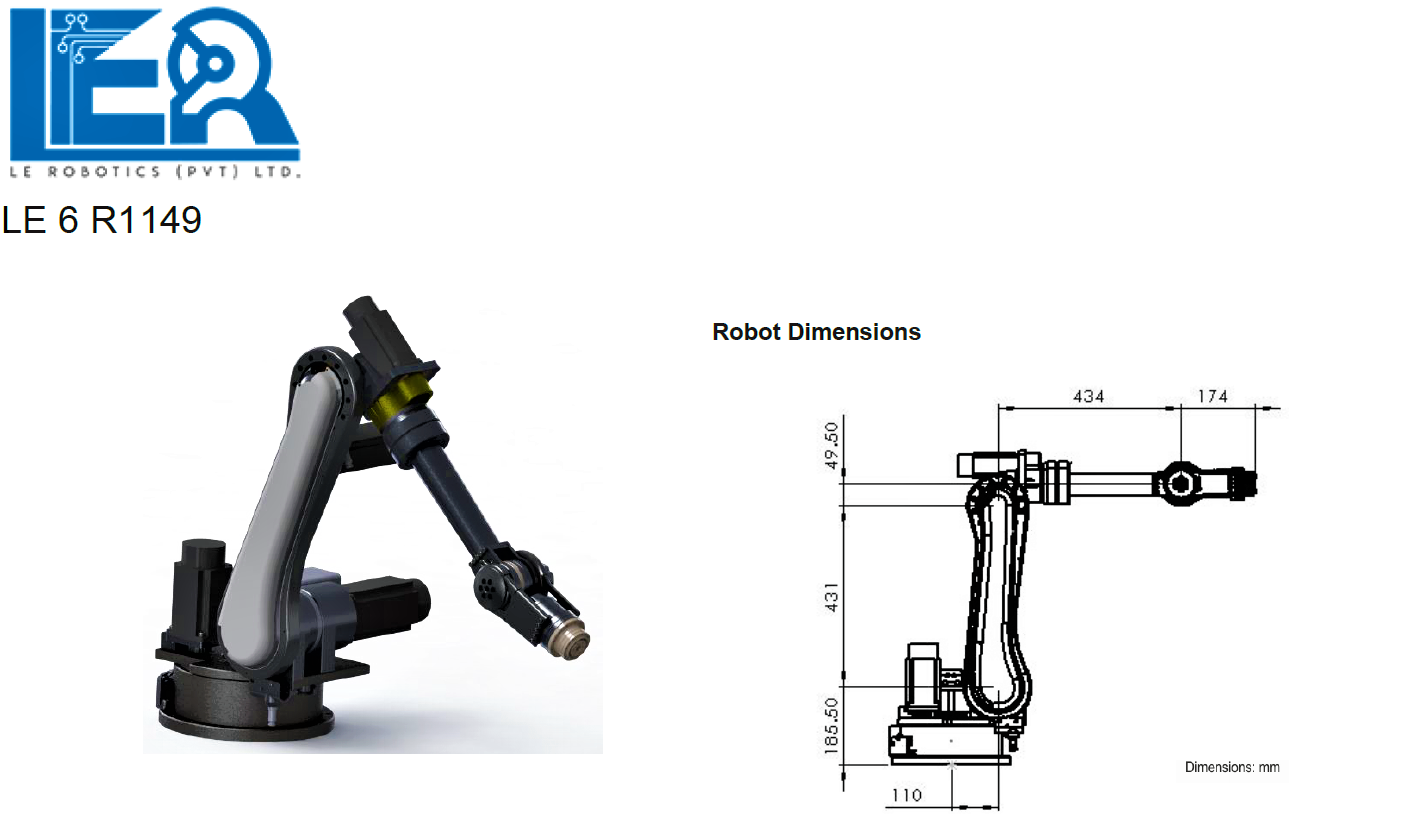
\includegraphics[width=0.7\linewidth]{figures/robots/sixdofrobot}
		}
		\caption{Model \textit{LE 6 R1149} 6-DOF articulated robot arm\cite{articlulated_robots}}
		\label{fig:sixdofrobot}
	\end{figure}
	
	
	
	\item\textbf{ 4 DOF Robots} - Robots with four degrees of freedom (Figure \ref{fig:fourdofrobot} depicts such a model)
	\begin{itemize}
		\item Robotics solutions with superior high-speed performance, high rigidity and high accuracy
		\item Array of options with a compact design
		\item Around 500 mm reach and 0.1 mm placement precision
	\end{itemize}

	\begin{figure}[h]
		\centering
		\fbox{
			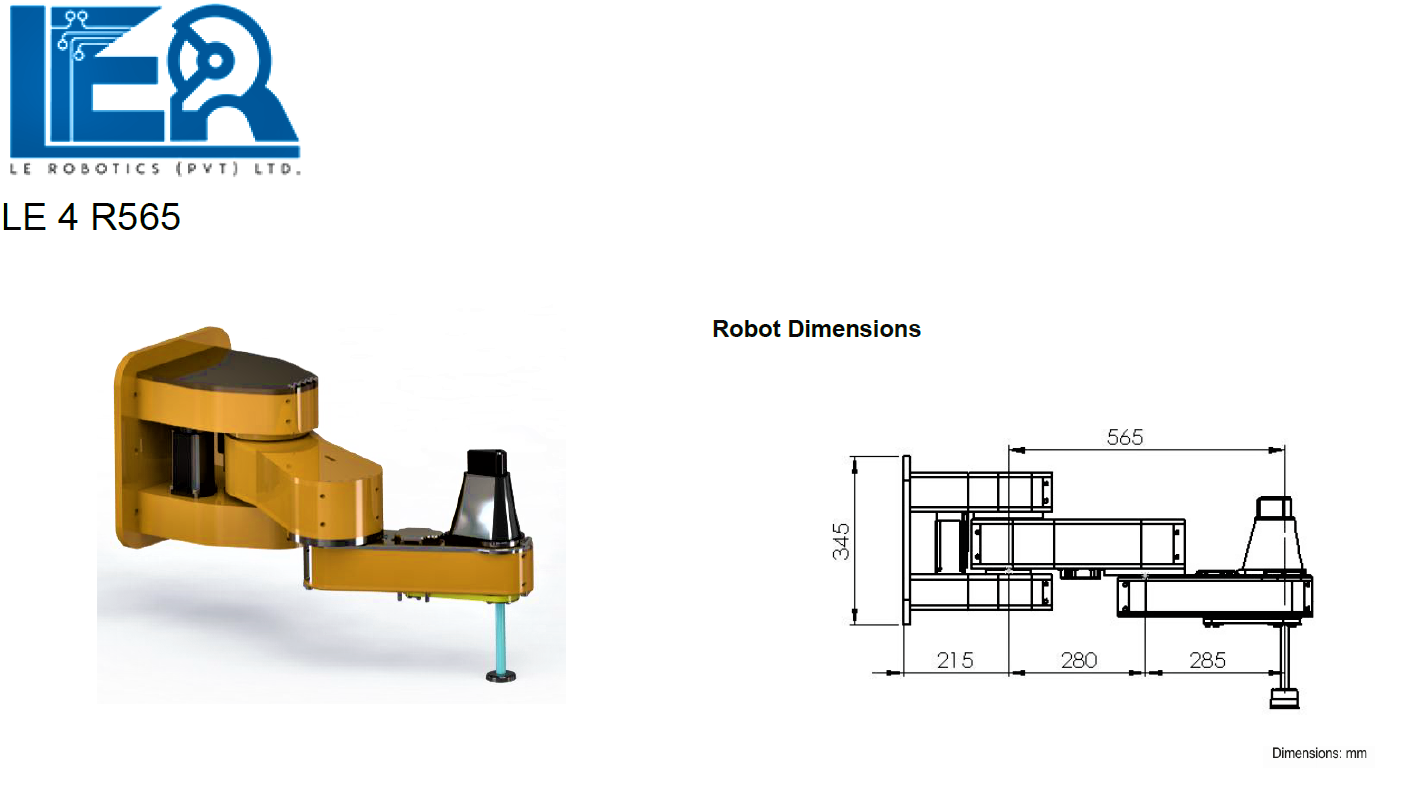
\includegraphics[width=0.7\linewidth]{figures/robots/fourdofrobot}
		}
		\caption{Model \textit{LE 4 R565} 4-DOF \ac{scara} robot arm\cite{scara_robots}}
		\label{fig:fourdofrobot}
	\end{figure}
	
	
	
	\item \textbf{Custom Made Robots} - Robots designed according to the customer's needs
	\begin{itemize}
		\item Reach and Payload specifications are possible to be customized as per your process requirements
		\item Robotics Solutions to carry out simple pick and place operations
	\end{itemize}
\end{enumerate}

\section{Past, Present and Future}
\label{Past Present and Future}
LE Robotics Pvt. Ltd. has been originally established as the \ac{rnd} division of its parent organization, Lanka Electronics (Pvt) Ltd. Lanka Electronics (Pvt) Ltd has been founded in 1993  by a group of graduates of the University of Moratuwa, the leading technical college in Sri Lanka. In 1993 they established their first electronic product manufacturing facility in the city of Minuwangoda and currently they own another manufacturing facility in Anuradhapura city.\\

Being a leading innovation company in Sri Lanka, Lanka Electronics (Pvt) Ltd has manufactured professional electronic devices for the Sri Lankan government and multinational companies such as \textit{Variosystems (Pvt) Ltd}. In chronological order, some of the professional electronic products they have manufactured so far are shown in Table \ref{table:pastproducts}. In addition to those, the company manufactures several consumer electronic products as well. TV antennas and Boosters are the mainstream consumer electronic products.

\begin{table}[h]
	\captionsetup{font=sc, labelsep=newline}
	\centering
	\caption{Professional electronic products of Lanka Electronics (Pvt) Ltd.}
	\begin{tabular}{|p{0.1\linewidth}  |p{0.7\linewidth}  |}
		\hline
		\textbf{Year} & \textbf{Product}\\\hline
		1993 & Laboratory training panels: discontinued manufacturing in 2010\\\hline
		1996 & Die-Sink \ac{edm} Machine: the first \ac{edm} machine built in Sri Lanka using 100\% locally developed technologies and local resources\\\hline
		1997& Motor Traffic Control Lights: the first traffic light system, that was built in Sri Lanka using local technologies and resources as per a request from the Sri Lankan government.\\\hline
		2009& Wire Winding Machines: manufactured for special request made by Variosystems (Pvt) Ltd.\\
		
		\hline
	\end{tabular}
	\label{table:pastproducts}
\end{table}

In present, none of the products mentioned in the Table \ref{table:pastproducts} are in production and the mainstream professional electronic product of the company is customisable industrial articulated robot arms. In addition to that related technologies such as servo motors, servo motor controllers and motor encoders  are researched and developed within the facility.

\chapter{Description of familiarization work carried out}
%2.4 of janiths report
\section{Projects Assignment}

Although the official internship period commenced on Tuesday $4^{th}$ of January in 2022, we had had our first meeting with the supervisor about a month prior to that. The meeting was conducted online through a video conferencing platform due to the Covid 19 situation in the country. Figure \ref{fig:firstmeet} shows a moment captured during the meeting.

\begin{figure}[h]
	\centering
	
	\fbox{
		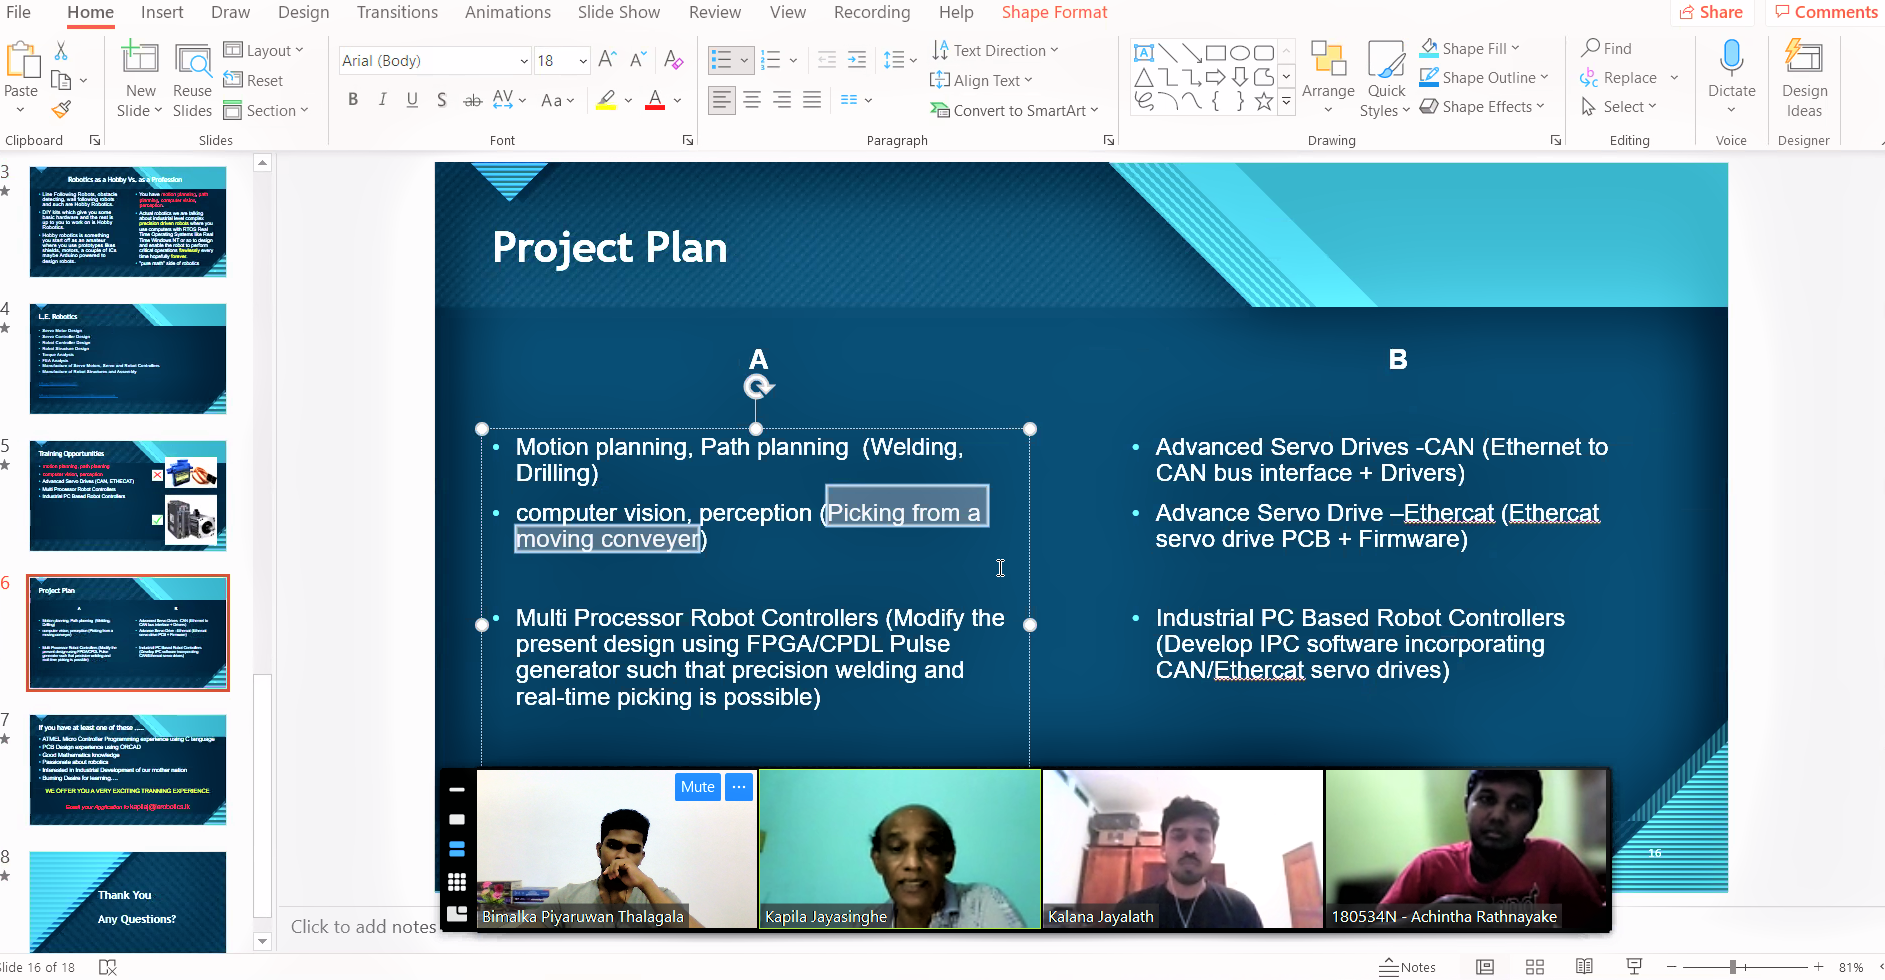
\includegraphics[width=0.9\linewidth]{figures/familiarization/projectplan}
	}
	\caption{First meeting with the supervisor to choose a project plan}
	\label{fig:firstmeet}
\end{figure}

In that meeting, our supervisor introduced the available projects that we can work on in our training period. He offered us two separate paths we can select to work during our internship period as described in Table \ref{table:familiarize}. Depending on our interests, we chose  `Plan A' to continue with and I selected the project related to \ac{cv}. In summary, that project was about engineering a \ac{cv} subsystem to integrate with an existing pick and place machine to pick objects from a moving conveyor belt.



\begin{table}[h]
	\captionsetup{font=sc, labelsep=newline}
	\centering
	\caption{Plans we were offered prior to beginning our industrial training}
	\begin{tabular}{|p{0.45\linewidth}  |p{0.45\linewidth}  |}
		\hline
		\textbf{Plan A} & \textbf{Plan B}\\\hline
		Motion planning, Path planning (welding, drilling) & 
		Advanced servo drivers - \Ac{can} (Ethernet to \ac{can} bus interface + Drivers)\\ \hline
		
		\ac{cv}, Perception (picking objects from a moving conveyor) &
		Advanced servo drive - Ethercat (Ethercat servo drive \ac{pcb} + Firmware)\\ \hline
		
		Multiprocessor robot controllers (modify the present design using \ac{fpga}/ \ac{cpld} pulse generator such that precision welding and real-time picking is possible)& 
		Industrial \ac{pc} based robot controllers (Developed \ac{ipc} software incorporating \ac{can}/ Ethercat servo drivers)\\
		\hline
	\end{tabular}
	\label{table:familiarize}
\end{table}

\section{Facility Familiarization}

LE Robotics Pvt. Ltd. is a fully featured \ac{rnd} facility located in Minuwangoda, Sri Lanka. Facility consists of most of the machinery required for industrial robot arm designing, including a \ac{cnc} machine, a Lathe machine, a Milling machine and various other machines. In addition to that facility has the resources for single side \ac{pcb} designing and testing. On the first day that we visited the facility, we were accompanied around it to see the various machines and electronic test instruments. Our supervisor gave brief descriptions about most of such tools and encouraged us to learn how to operate them in our free time.\\

\section{Introduction to Industrial Robot Arm Designing}

On the same day, Supervisor gave us an explanation about the evolution of already developed industrial robot arms that were described in the Section \ref{Services and Products}. The explanation included capabilities and drawbacks of each design as well as the advantages and disadvantages of incorporating third party technologies to manufacture them locally.\\

Then he explained the importance of manufacturing all the parts of an industrial robot arm within the facility rather than simply using the available parts. Because then the manufacturer has the full potential to customize any design to best fit to a given application. If the third party parts are used this customization capability is reduced drastically and we have to adjust our designs just to suit them rather than the application. Due to this reason, LE Robotics Pvt. Ltd. has taken a great initiative to manufacture different types of motors locally using the available materials and knowledge.

\section{Non-Disclosure Agreement}

Another important concept that the supervisor pointed out on the familiarization session was \ac{nda}. It is a legal contract or part of a
contract between at least two parties, that outlines confidential material, knowledge, or information that the parties wish to share with one another for certain purposes but wish to restrict access to\cite{nda}. An \ac{nda} document contains the details given below.

\begin{enumerate}
	\item Definitions of the terms used in the document such as Confidential Information, Disclosing Party and Receiving Party.
	
	\item Rules and regulations related to Use, Disclose and Reproduce the shared confidential information.
	
	\item Actions to be taken in an event of breach of a term of the agreement mentioned in the previous point.
	
	\item Non-Competition Clause which emphasizes the requirement	of a written permission prior to	direct or indirect attempt to register	or use the Disclosing Party’s	confidential information, during the	term of the agreement and the expiry of the agreement.
	
	\item Governing Law which describes the way of interpreting the agreement.
	
	\item Confidentiality Period/ Termination which specifies the duration of time	that the agreement remains in	force, if its is not terminated earlier	in writing by mutual agreement.
\end{enumerate}


Since we were temporary employees of the company we did not have access to any of the trade secrets of LE Robotics Pvt. Ltd., such as hardware blueprints, software source codes and etc. Therefore, the supervisor mentioned that  there  was no requirement to sign an \ac{nda}. However, he explained the importance of obeying an \ac{nda} as a professional engineer.


\chapter{Exposure to Other Departments}

As we could observe, most of the operations related to various departments of the LE Robotics (Pvt.) Ltd. is carried out by its parent company which is `Lanka Electronics (Pvt) Ltd.' introduced in Section \ref{Past Present and Future}. That is departments of the parent company handle the operation of the LE Robotics (Pvt.) Ltd. as well. As we were recruited only to the LE Robotics (Pvt.) Ltd we were not exposed to the detailed operations of other departments such as HSE, Finance, Administration and Logistics. 

\section{Finance Department}

Finance Department is the entity in an organization which is responsible for handling money on behalf of the company. It carries out the operations such as accounting, preparing and forecasting budgets, examining financial statements and etc. During our internship, we were not exposed to such activities in the finance department of LE Robotics (Pvt.) Ltd. The only visible interaction with the financial department and the interns was receiving the monthly wages on the specified date.\\

From the very beginning,  I was instructed and encouraged to incorporate open source technologies as much as possible to develop my assigned project to avoid the cost of licenses. Otherwise, the company has to pay for various commercial grade licenses which can simply overflow their allocated budget for my project.  Such strategies taught me how to develop viable products while staying within the budget. In addition to that, my supervisor highlighted the importance of properly documenting the work done. Because if I do not do so, the next employee who will undertake my project, has to start from scratch to understand my project and it will be a loss for the company in terms of both money and time.


\section{Logistics Department}

Logistics department holds the responsibilities related to management of the flow of materials/ products from a point of origin to a point of consumption. Since LE Robotics (Pvt.) Ltd. is a \ac{rnd} facility which manufactures highly tech industrial instruments, required electronic components are imported directly from international electronic component distributors such as \textit{Digi-Key Electronics} and \textit{Farnell}. Company closely work with international logistic services such as FedEx to get the required components to their doorstep.

%===========================================================================
\chapter{Project Work}
\label{Project Work}
By title, the project that I was assigned, was \textbf{\textit{Machine vision based Real-time Motion Planning for an Industrial Articulated Robot Arm}}. In simple words, it was a project related to an automatic pick and place machine which can be used to pick objects placed on a conveyor belt and pass them to the next stage of processing.\\

My contribution to that project was to develop the following three aspects of the system. 

\begin{enumerate}[I.]
	\item Development of an object detection framework
	
	\item Development of an application for camera calibration (referred as \textit{Camera Calibrator \ac{gui}} in this document)
	
	\item Development of an application to train an object classification model (referred as \textit{Classifier Trainer \ac{gui}} in this document)
	
\end{enumerate}

Subsequent sections explain the mentioned sub-projects that were undertaken by me during the industrial training period. Implementation details are not exposed in this report as it does not comply with professional engineering ethics.



\section{Development of an Object Detection Framework}
\label{Development of an Object Detection Framework}
The first project, that I was assigned as a trainee electronic engineer was related to the \ac{cv} field. In this project, an Object Detection Framework was developed to be deployed in an Automatic Pick and Place Machine. In a summary, the framework is capable of identifying \ac{roi}, detecting and classifying objects, and determining the location and orientation of objects with respect to a real-world coordinate system for grasping (picking). This section explains everything related to the development of that framework.


\subsection{Problem Definition}\label{Problem Definition}
Most of the robotic arms used in industrial environments operate in a pre-programmed cycle. When comes to the way a human does the same task is much different as the path planning for picking an object may change from cycle to cycle because of the perception obtained through human vision. \Ac{cv} is the technology and methods incorporated to mimic the human vision in order to gain insights into the operating environment of the robotics system.\\

When it comes to real-time object detection using \ac{cv}, there is an inevitable trade-off between the accuracy and the speed of the operation. This depends entirely on the used \ac{cv} algorithms and the computational power of the available hardware. If the robotic system/ arm in interest is not controlled through a dedicated industrial PC with adequate computational resources, the amount of resources that can be allocated to the \ac{cv} unit becomes limited.  This will eventually result in great delays (which is not desirable when it comes to real-time operations) to produce the required outputs by processing the acquired images through the associated camera.\\

Due to the limitations in the resources, the initial problem of real-time object detection on a moving conveyor was subdivided into three problems.

\begin{itemize}
	\item \textbf{Case 1:} Detection of objects placed in a \textbf{\textit{static environment}} (no conveyor belt is associated). Picking and placing is carried out by the robot in the usual way.
	
	\item  \textbf{Case 2:} Detection of objects placed on a \textbf{\textit{non-continuous conveyor belt}}. The conveyor belt can be paused when objects are detected and picking and placing is carried out thereafter.
	
	\item \textbf{Case 3:} Detection of objects placed on a \textbf{\textit{continuously moving conveyor belt}}. Picking and placing happen while the conveyor is moving.
\end{itemize}



\subsection{Solution}
\label{cv_subsystem}
As the initial stage of the project, case 1 mentioned in Section \ref{Problem Definition} was developed. It consisted of developing a \ac{cv} subsystem for detecting \textbf{\textit{stationary objects}} placed in a \textbf{\textit{static environment}}. In this case, no conveyor belt is used and objects are placed in the \ac{fov} of the camera.\\

Figure \ref{fig:ioprocess} shows the interconnection between inputs and outputs of the developed system. Once the video stream from a camera is fed into the system, it is capable of,



\begin{enumerate}
	\item Determining the grasping location of an object in a real-world coordinate system. The centroid of the 2D view of the object was considered as the grasping location. 
	
	\item Determining the gripper's angle. Orientation of object with respect to the positive x direction of the same real-world coordinate system was used for this.
	
	\item  Determining the class/ type of the detected objects using a \ac{sift} and \ac{svm} based classification algorithm.
\end{enumerate}

and providing them to the main controller of the pick and place machine as requested by it.\\ 

\begin{figure}[h]
	\centering
	
	\fbox{
		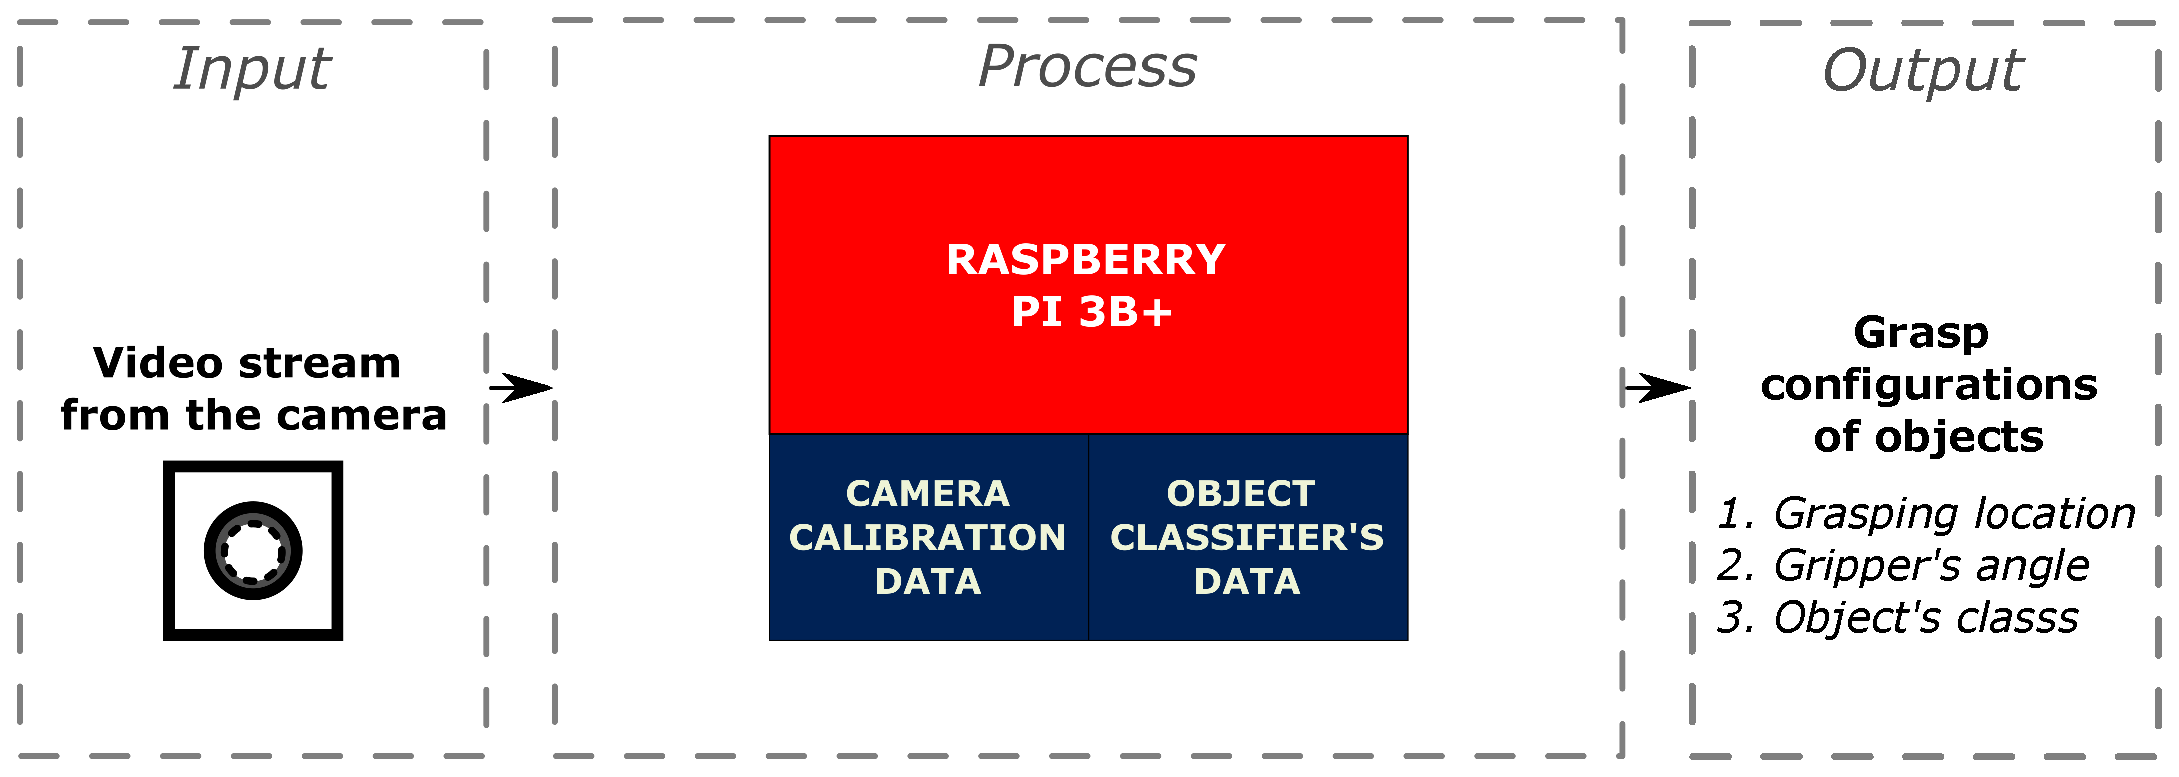
\includegraphics[width=0.8\linewidth]{figures/system/ioprocess.eps}
	}
	\caption{Interconnection between inputs and outputs of the \ac{cv} subsystem}
	\label{fig:ioprocess}
\end{figure}



Figure \ref{fig:cvsubsys} depicts the interconnections between the existing robot controller and the newly developed computer vision subsystem. Outputs shown in Figure \ref{fig:ioprocess} are provided to the robot controller through a serial communication link built using an \ac{uart} circuitry. For transferring data to the Raspberry Pi from the working PC, \ac{sftp} over Wi-Fi technology was used.

\begin{figure}[h]
	\centering
	
	\fbox{
		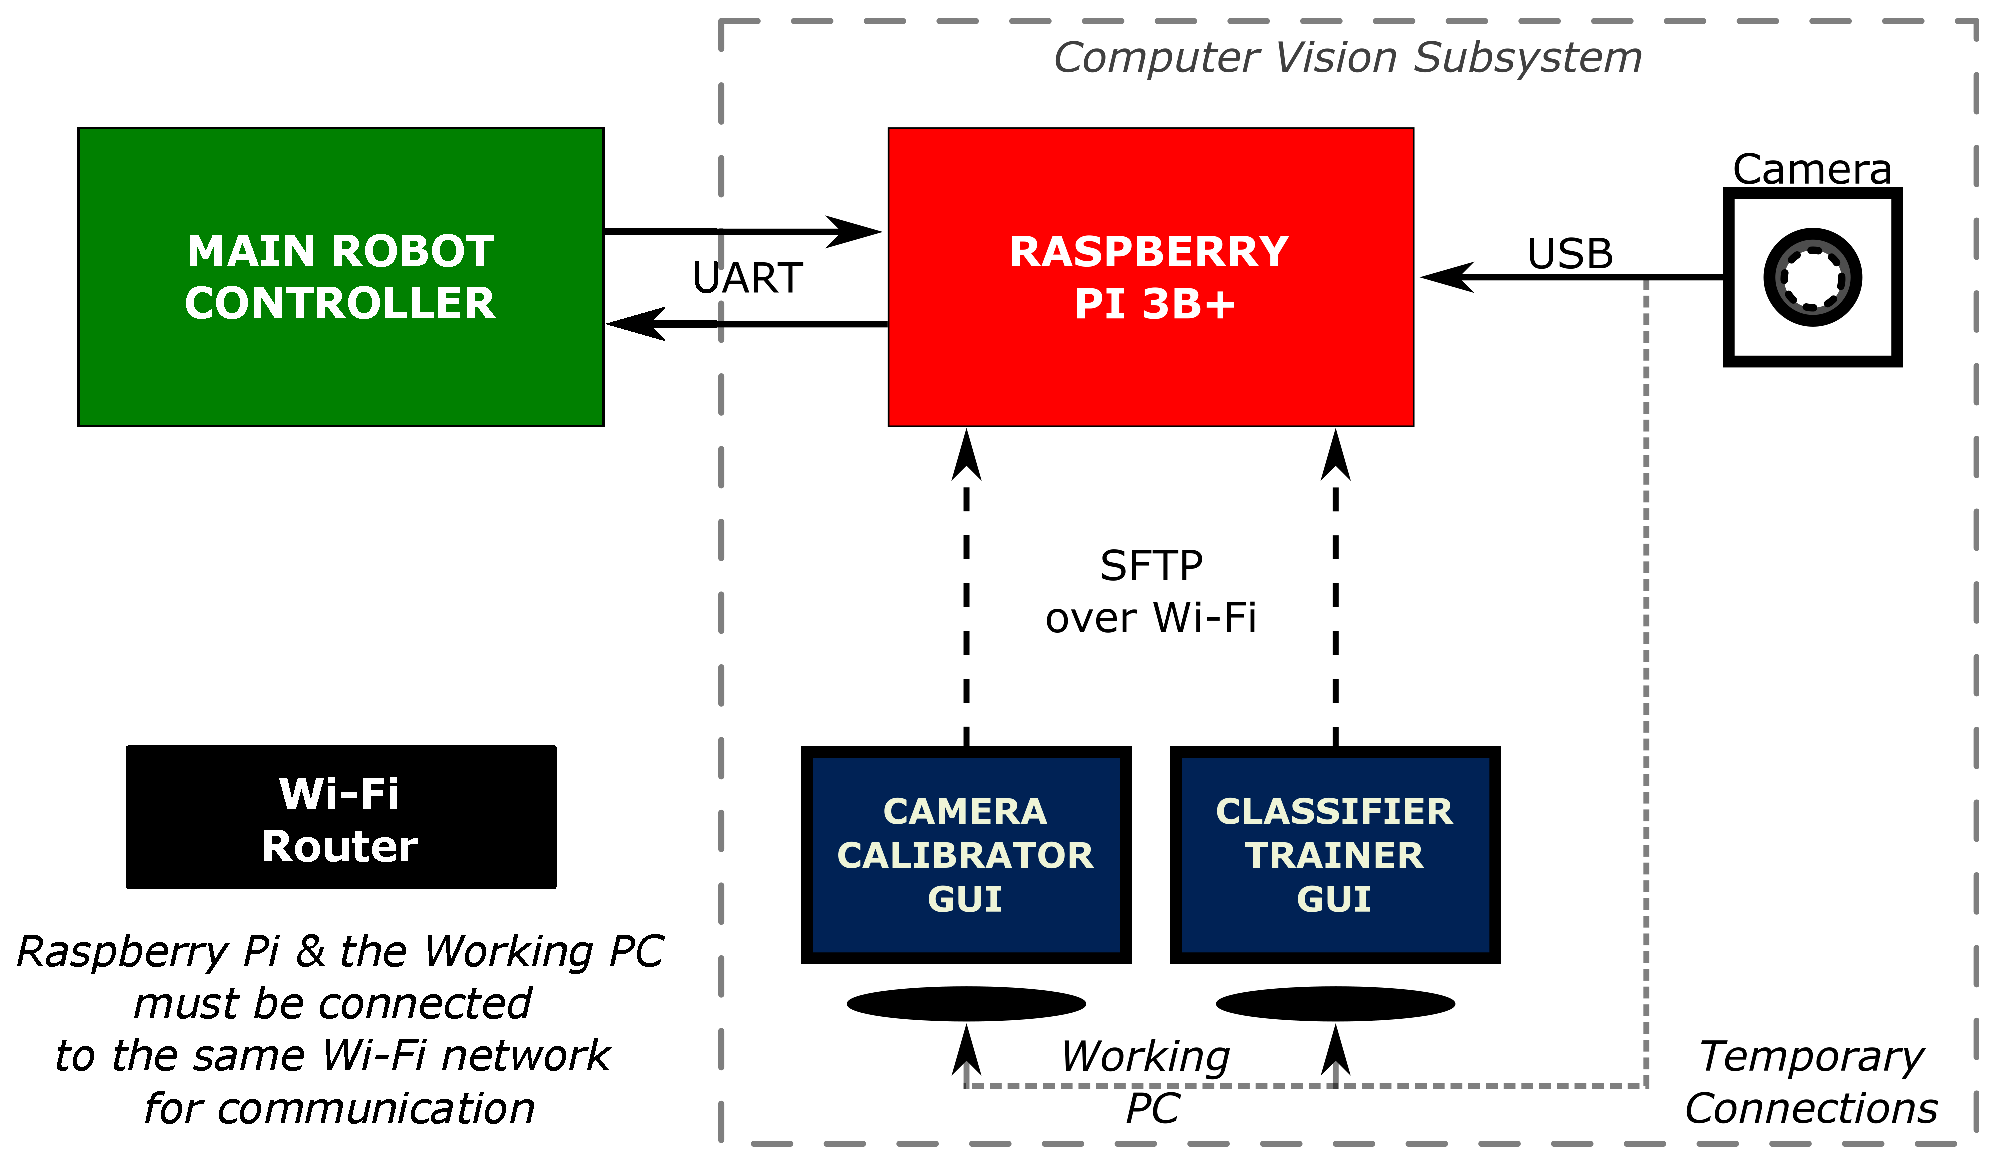
\includegraphics[width=0.8\linewidth]{figures/system/system.eps}
	}
	\caption{Interconnections between the existing robot controller and the \ac{cv} subsystem}
	\label{fig:cvsubsys}
\end{figure}

For the implementation of the prototype, third-party tools given below are used.\\

\begin{enumerate}[1.]
	\item \textbf{\ac{rpi} 3 B+ Single Board Computer (SBC)}\\
	\textit{Product brief:} Online available at \url{https://datasheets.raspberrypi.com/rpi3/raspberry-pi-3-b-plus-product-brief.pdf}.
	
	\item \textbf{Logitech C310 HD Webcam, 720p Video}\\
	\textit{Technical specifications:} Online available at \url{https://support.logi.com/hc/en-us/articles/360023464573-Logitech-HD-Webcam-C310-Technical-Specifications}.
	
	\item \textbf{OpenCV open source computer vision library stable release 4.4.0}\cite{opencv_library} \\
	\textit{Stable and development releases:} Online available at \url{https://github.com/opencv/opencv}; A pre-compiled version of this library, which is optimized for \ac{cv} and Deep Learning on Raspberry Pi was used.
	
	\item \textbf{Gordon's Arduino wiring-like WiringPi Library for the Raspberry Pi}\cite{wiringpi} \\
	\textit{Unofficial Mirror for WiringPi bindings:} Online available at \url{https://github.com/WiringPi/WiringPi}.
	
\end{enumerate}


During the operation of the pick and place robot, the developed object detection algorithm runs only inside the \ac{rpi}. However, for the operation of that algorithm, it requires the data shown in Table \ref{table:datafiles}. A Windows \ac{gui} was developed to generate those data and the `Description' column of Table \ref{table:datafiles} provides only a simple overview of that data . Subsequent sections explain the functionality and the working principles of the mentioned \ac{gui}, in detail.\\

\begin{table}[h]
	\captionsetup{font=sc, labelsep=newline}
	\centering
	\caption{ Data files required to run the object detection framework}
	\begin{tabular}{|p{0.3\linewidth}  |p{0.6\linewidth}  |}
		\hline
		\textbf{File Name} & \textbf{Description}\\\hline
		{\tt calibration\_data.xml} & This file includes camera calibration data. That is, intrinsic and extrinsic parameters of the associated camera.\\ \hline
		{\tt objects\_data.xml} & This file includes object classification model's data. That is, the data required for the object classification (class names, trained support vector machines and etc.).\\
		\hline
	\end{tabular}
	\label{table:datafiles}
\end{table}





\section{Development of an Application for Camera Calibration}
\label{Development of an Application for Camera Calibration}
The second project, that I was assigned as a trainee electronic engineer was related to the \ac{se} field. In this project, a Windows \ac{gui} was developed to calibrate a given camera. In a summary, the application is capable of generating the required data, to remove the distortions of captured images and to transform 2D image points back to a given 3D real-world coordinate system with an accuracy of $\pm 0.5 ~mm$.

\subsection{Problem Definition}

The end goal of the \ac{cv} subsystem mentioned in the Section \ref{cv_subsystem} is to provide the location and orientation of the identified objects, with respect to a known real-world coordinate system. However, when an image is captured, the details about the depth of the object relative to the camera are lost due to the real world to image plane transformation (the forward projection \cite{hartley_zisserman_2004}) happens inside the camera. This operation is non-invertible.\\

There are several methods used in \ac{cv}  literature to back-project image plane coordinates to the real-world coordinate system. In this project, a method which uses a single calibrated camera and analytic geometry was implemented. It was observed that the back-projected coordinates are accurate at least to $\pm 0.5 ~mm$. As mentioned for this back-projection process, a \textit{calibrated camera} is required and the rest is engineering mathematics. Therefore, the actual problem to be solved was to calibrate the camera associated with the pick and place machine.



\subsection{Solution}
Camera Calibration refers to the extraction of various parameters related to the camera that will be used to capture the video stream/ images. These parameters are required when the back-projection is done. For the camera calibration, the method that uses an asymmetric chess board was used\cite{cam_calib:_nodate}. Because that method was really simple and could be implemented easily using the resources that were available in the facility. The process of camera calibration is given in the Appendix \ref{Camera Calibration}.\\

Once the camera calibration is done, we will be able to extract the intrinsic and extrinsic parameters of a given camera. Those parameters can then be used for back-projection which was my problem at hand. Extracted intrinsic parameters which are specific to the  used  camera, do not depend on the image. Among those parameters, \textit{Camera Matrix} is what has the greatest important. \textit{Radial/ Tangential Distortions} have a minimal importance and therefore can be neglected. Extracted extrinsic parameters of the image shown in Figure \ref{fig:backprojectimage}  are specific for that image. If in any case, orientation or the place of the camera is altered, these must be recalculated in order to be used in the back-projection algorithm.\\
	
	
As mentioned previously ultimate goal of this sub project was to develop a \ac{gui} application for camera calibration. The process mentioned above was therefore implemented in {\tt C\#} programming language using `\textit{Visual Studio 2019}' software. For the implementation, the \textit{Emgu CV} library which is a cross platform \textit{.Net} wrapper to the OpenCV image processing library was also used. It allows OpenCV functions to be called from .NET compatible languages like {\tt C\#} and therefore make the software development process efficient. The developed \ac{gui} is shown in the Figure \ref{fig:calibgui}.

\begin{figure}[h]
	\centering
	\fbox{
		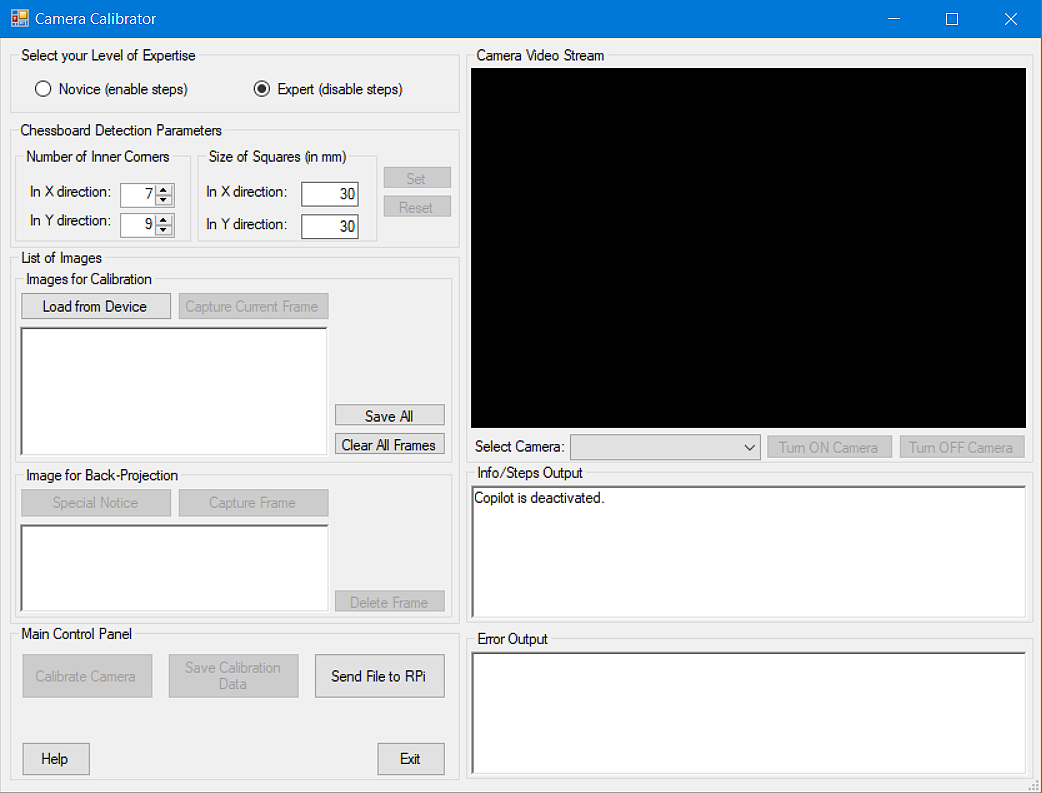
\includegraphics[width=0.8\linewidth]{figures/calib/gui}
	}
	\caption{Camera calibrator \ac{gui} for Windows}
	\label{fig:calibgui}
\end{figure}

Once the camera calibration is done, the software can also be used to send the file that includes the necessary data to the \ac{rpi}. For that the \ac{rpi} and the working \ac{pc} where the software is run,  must be connected to the same \ac{lan} over WiFi.


\section{Development of an Application to Train an Object Classification Model}
\label{Development of an Application to Train an Object Classification Model}
The third project, that I was assigned as a trainee electronic engineer was also related to the \ac{se} field. In this project, a Windows \ac{gui} was developed to train a \ac{ml} model which can be used classify set of pre-defined objects. In a summary, the application is capable of generating the required data, to classify identified objects by the object detection framework explained in the Section \ref{Development of an Object Detection Framework}. Figure \ref{fig:classification} shows how the object detection framework classifies objects with the help of object classification model.

\begin{figure}[h]
	\centering
	\fbox{
		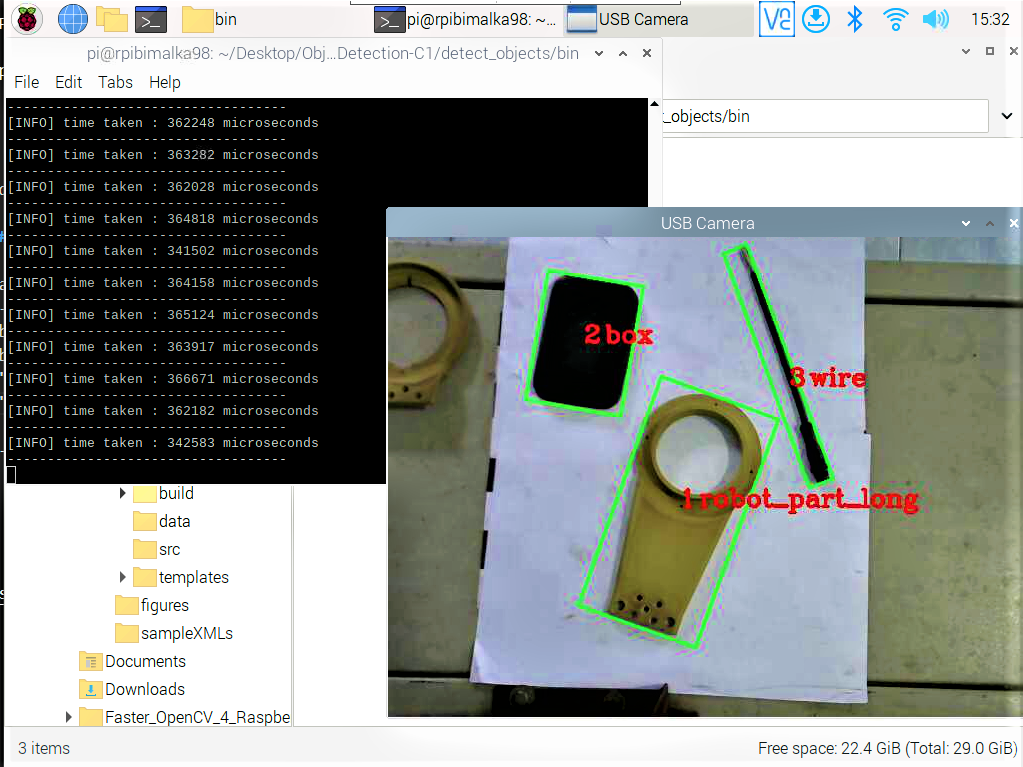
\includegraphics[width=0.8\linewidth]{figures/odf/v3siftsvm}
	}
	\caption{Output of the object detection framework with object classification capability}
	\label{fig:classification}
\end{figure}


\subsection{Problem Definition}

One of the key aspects of an object detection framework is to classify the detected objects. Because, in order to effectively make use of the information of the detected objects, it is necessary to know the type/class of them. In \ac{cv} literature there are various methods to determine the class of a detected object. Accuracy as well as the speed of the predictions was a major concern when selecting a method, as the end product was supposed to use in an industrial environment. By considering all of such aspects it was decided to use an \ac{ml} model which is based on \ac{sift} features and \ac{svm}s.


\subsection{Solution}

Prior to deploy any \ac{ml} tool for predictions in any system, they must be trained for the target task by feeding it the necessary data. In literature this task is known as \textit{training an \ac{ml} model}. Similarly, in our case the object classification model must be trained prior to couple it with the object detection framework explained in the Section \ref{Development of an Object Detection Framework}. This training phase of the classification model is carried out using a Windows \ac{gui} application developed using Emgu CV (a cross platform .Net wrapper to the OpenCV image processing library) package\cite{emgucv}. Figure \ref{fig:classtrainer} depicts the layout of the designed Windows \ac{gui}.\\

\begin{figure}[h]
	\centering
	\fbox{
		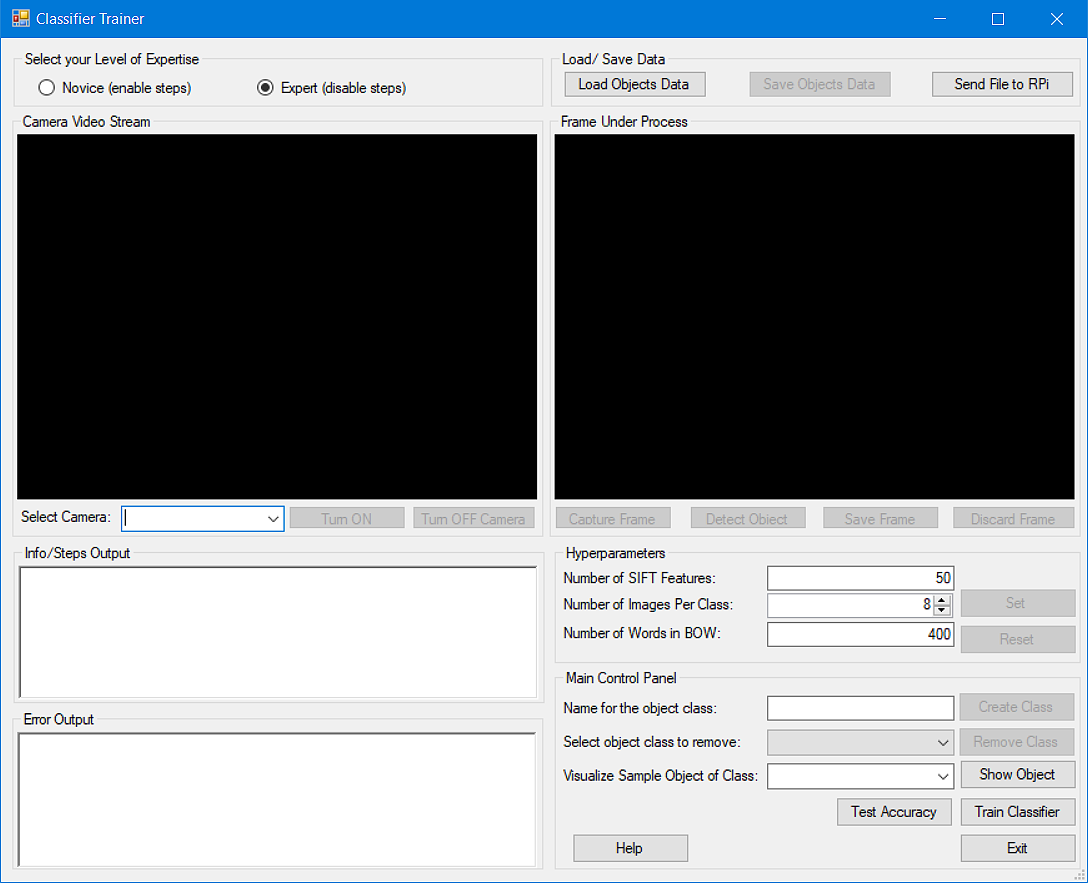
\includegraphics[width=0.8\linewidth]{figures/ml/classifiergui}
	}
	\caption{Classifier trainer GUI for Windows}
	\label{fig:classtrainer}
\end{figure}

Once the training is done, the software can also be used to test the accuracy of the prediction model to fine tune its performance. Ultimately, the file that includes the necessary data can also be sent to the \ac{rpi} using the same software. For that the \ac{rpi} and the working \ac{pc} where the software is run,  must be connected to the same \ac{lan} over WiFi.\\

When the model is trained on a set of object classes, we can keep using the model for classification as long as we do not introduce new objects classes to our object detection framework.In addition to that, \ac{svm}s were trained using the one-vs-all approach. Therefore, each object class has its own \ac{svm} which decides whether an object belongs to that class or not (a binary classification problem). Therefore, the calculated histogram of features, of a given \ac{roi} (an object) is passed through all of \ac{svm}s when deciding the class of an object. This improves the accuracy of predictions but sacrificing the time. Therefore, time it takes to run a single object detection routine will depend on two factors.

\begin{enumerate}
	\item Number of non overlapping objects placed in the \ac{fov} of the camera: \textit{Higher the number of objects, longer the time object detection takes.}
	
	\item Number of classes of objects: \textit{Lesser the number of classes  shorter the time object detection takes.}
\end{enumerate}



%===========================================================================
\chapter{Hands-on experiences}

The entire six months period of my industrial training was full of hands-on experiences. It was an ideal combination of learning, unlearning and relearning. LE robotics Pvt. Ltd. had no experts in the \ac{cv} field during the time I was working there. Therefore, I had to learn most of the things related to my assigned projects by actually doing them. This made an ideal opportunity for me to learn various technologies really fast and with minimum supervision. 

\section{Resources for Self-Learning}

As I made a lot of design decisions on my own while doing the project, I had to extensively refer to various knowledge resources throughout my training period. This taught me the right skill set to identify reliable information sources among a lot of garbage on the internet. Following is a list of information sources that I used during my training.\\

\begin{itemize}
	\item Google Search 
	\item Stack Overflow 
	\item OpenCV Documentations 
	\item EmguCV Documentations 
	\item Research Publications
\end{itemize}

\subsection{Google Search}

\textbf{Website}: \url{https://www.google.com/}

Without any doubt, the starting point of exploring any information on internet was the \textit{Google Search}.  It is the search engine provided by Google. The power of modern google search is pretty amazing and it can quickly adapt to your search patterns. This lets it bring the most relevant information to the user. Therefore, using the correct terms during a search matters and the quality of retrieved information extensively depends on that.

\subsection{Stack Overflow}

\textbf{Website}: \url{https://stackoverflow.com/}

\textit{Stack Overflow} is a question and answer website for professional and enthusiast programmers. It features questions and answers on a wide range of topics in computer programming\cite{stackoverflow}. If you are not doing something really new that no one has ever done, there's a high probability of finding an answer to any question which you may come across. Stack Overflow is that rich of various solutions to fit exactly to your problem at hand.\\

Additionally, the number of \textit{Scores} an answer has obtained for a particular question is an ideal measure to estimate the the reliability of the answer. Moreover, answers can be easily linked in your documentations and source codes using their associated \textit{Share} links. Figure \ref{fig:stackof} depicts an answer to a question asked on the Stack Overflow platform. The actual answer is available at \url{https://stackoverflow.com/a/10230489/15939357}.

\begin{figure}[h]
	\centering
	\fbox{
		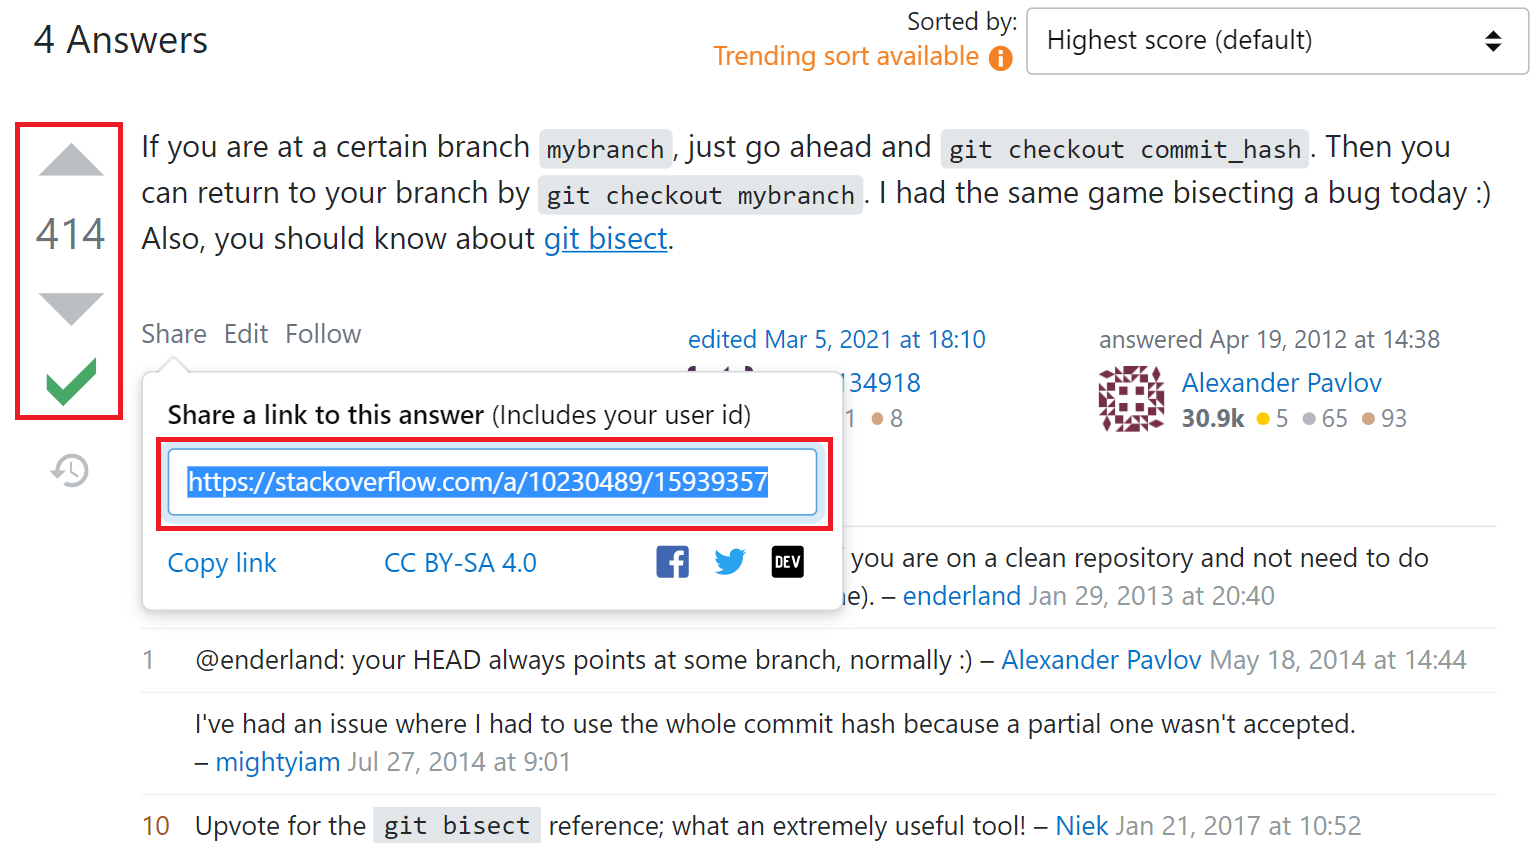
\includegraphics[width=0.7\linewidth]{figures/handson/stackof}
	}
	\caption{A sample answer on Stack Overflow and its associated shareable link}
	\label{fig:stackof}
\end{figure}

\subsection{OpenCV Documentations}

\textbf{Website}: \url{https://docs.opencv.org/4.x/}

OpenCV (Open Source Computer Vision Library: \url{http://opencv.org}) is an open-source library that includes several hundreds of computer vision algorithms. It also includes high quality documentation as well, for each module of the library. These documentation contains theoretical concepts and a vast amount of example code snippets. Such code snippets can be used to understand the way of using a particular function in a given application. 

\subsection{EmguCV Documentations}
\label{EmguCV Documentations}

\textbf{Website}: \url{https://www.emgu.com/wiki/index.php/Documentation}

EmguCV is a  cross platform .Net wrapper for the OpenCV image-processing library. It allows OpenCV functions to be called from .NET compatible programming languages like {\tt C\#}. The wrapper can run on Windows, Android, iOS, Mac OS and Linux. EmguCV also includes a rich documentation which explains usage of various functions and their interfaces. This documentation comes handy when it comes to Windows \ac{gui} development in {\tt C\#} using Visual Studio software.

\subsection{Research Publications}


Research publications are various documents published by academic institutes, research laboratories and other renowned companies such as Google, Microsoft and etc in the world. Therefore, the information on those publications is well documented and validated which makes them an ideal information source. In addition to that, their reliability is also very high as the authors are professionals in their respective fields. If you are working in a specific field and you want the most up-to-date knowledge in that field research publications are the tool to use. There is a vast number of websites which publish such articles and therefore they are not mentioned here.




\section{Usage of Open Source Software}

\subsection{Introduction}

\Ac{oss} is computer software that is released under a license in which the copyright holder grants users the rights to use, study, change, and distribute the software and its source code to anyone and for any purpose\cite{oss}. The purpose may be either commercial or private use. Most of the time such \ac{oss} are developed in a collaborative manner through  online platforms such as \textit{GitHub (\url{https://github.com/})} and general public has the access to examine the source codes. Additionally, any potential developer can contribute to such open source technologies and number of contributors has no limit.


\subsection{Advantages}

During our internship, we were encouraged  to use open source technologies as much as possible inside our project implementations. Because it has a lot of advantages when it comes to \ac{rnd} field. Few of them are listed below.

\begin{itemize}
	\item Most of the open source software are free of charge and there is no need of purchasing a license to use the source codes.
	
	\item Since \ac{oss} are developed in collaborative manner through publicly available online platforms, software are highly optimized due to the diverse perspectives of their developers. 
	
	\item There are  well established community driven online platforms to sort out different problems that may encounter during project development. Most of the time answers to such problems are readily available.
	
	\item Due to the indefinite number of contributors, there is a rich set of documentations related to the software. This makes the production really efficient as there is no need of blindly experimenting with the software.

\end{itemize}

The EmguCV docs that were introduced in the Section \ref{EmguCV Documentations} contain much description about functions in its library.
However, EmguCV docs does not contain code examples. This was a challenge  that I faced during the development of the software which were explained in the Sections \ref{Development of an Application for Camera Calibration} and \ref{Development of an Application to Train an Object Classification Model}. This is where the power of open source technologies can be used. EmguCV's source codes are hosted and developed at \url{https://github.com/emgucv/emgucv}. Therefore, they can be accessed by anyone without any charge and can be used to understand the usage of available functions in various applications. Situation is the same for OpenCV and its source codes are hosted and developed at \url{https://github.com/opencv/opencv}.\\

In addition to that, each such repository contains a section named as \textit{Issues} with various modifications requests and questions raised by the community. This issues section can be a life saver when working with latest versions of the software, as most of the problems that may encounter when using the latest versions may not be answered anywhere else on the internet. Figure \ref{fig:issues} depicts the issues section of the OpenCV project repository.


\begin{figure}[h]
	\centering
	\fbox{
		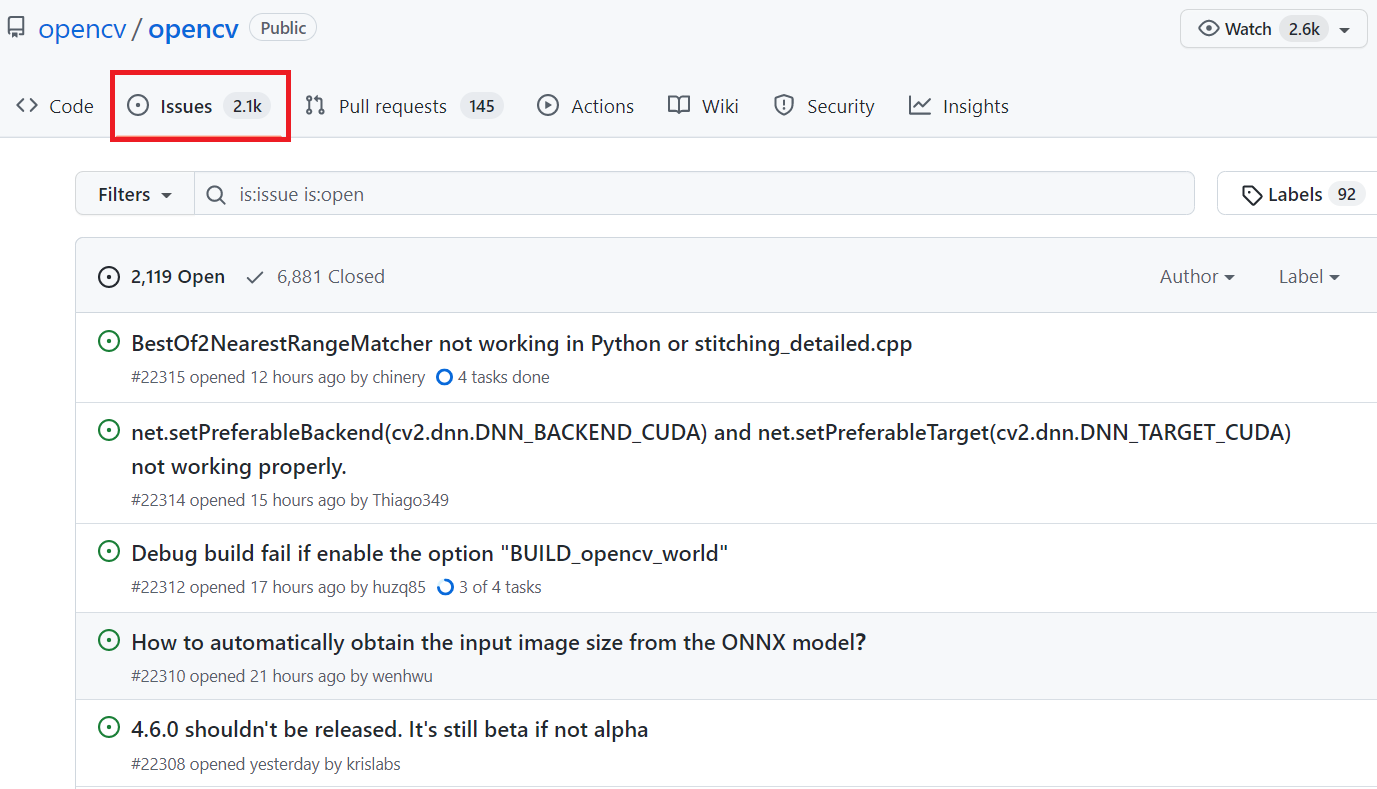
\includegraphics[width=0.7\linewidth]{figures/handson/issues}
	}
	\caption{Issues section of the OpenCV project repository}
	\label{fig:issues}
\end{figure}


\section{Usage of Modern Tools}

As described in the Section \ref{Project Work}, throughout my internship period I had to work with technologies related to \ac{cv} and \ac{se}. Therefore, I gained a lot experience of using various tools related to \ac{sdlc}. The tools I used can be classified into two categories depending on the area I used them. That classification is shown in the Table \ref{table:moderntools}.

\begin{table}[h]
	\captionsetup{font=sc, labelsep=newline}
	\centering
	\caption{Modern tools used during the development of the software}
	\begin{tabular}{|p{0.35\linewidth}  |p{0.35\linewidth}  |}
		\hline
		\textbf{Windows \ac{gui} Development} & \textbf{Object Detection Framework Development}\\\hline
		Visual Studio 2019 & Visual Studio Code\\
		Git & Git\\
		& CMake\\		
		\hline
	\end{tabular}
	\label{table:moderntools}
\end{table}
\pagebreak
\subsection{Visual Studio 2019}

\textit{Visual Studio 2019} is simply an \ac{ide} owns and developed by Microsoft. It provides necessary facilities for computer programmers to develop software. It consists of a source code editor, build automation tools, debugger and many more features that an \ac{ide} should contain \cite{vs2019}. Figure \ref{fig:vs} shows an instance of the application.\\

\begin{figure}[H]
	\centering
	\fbox{
		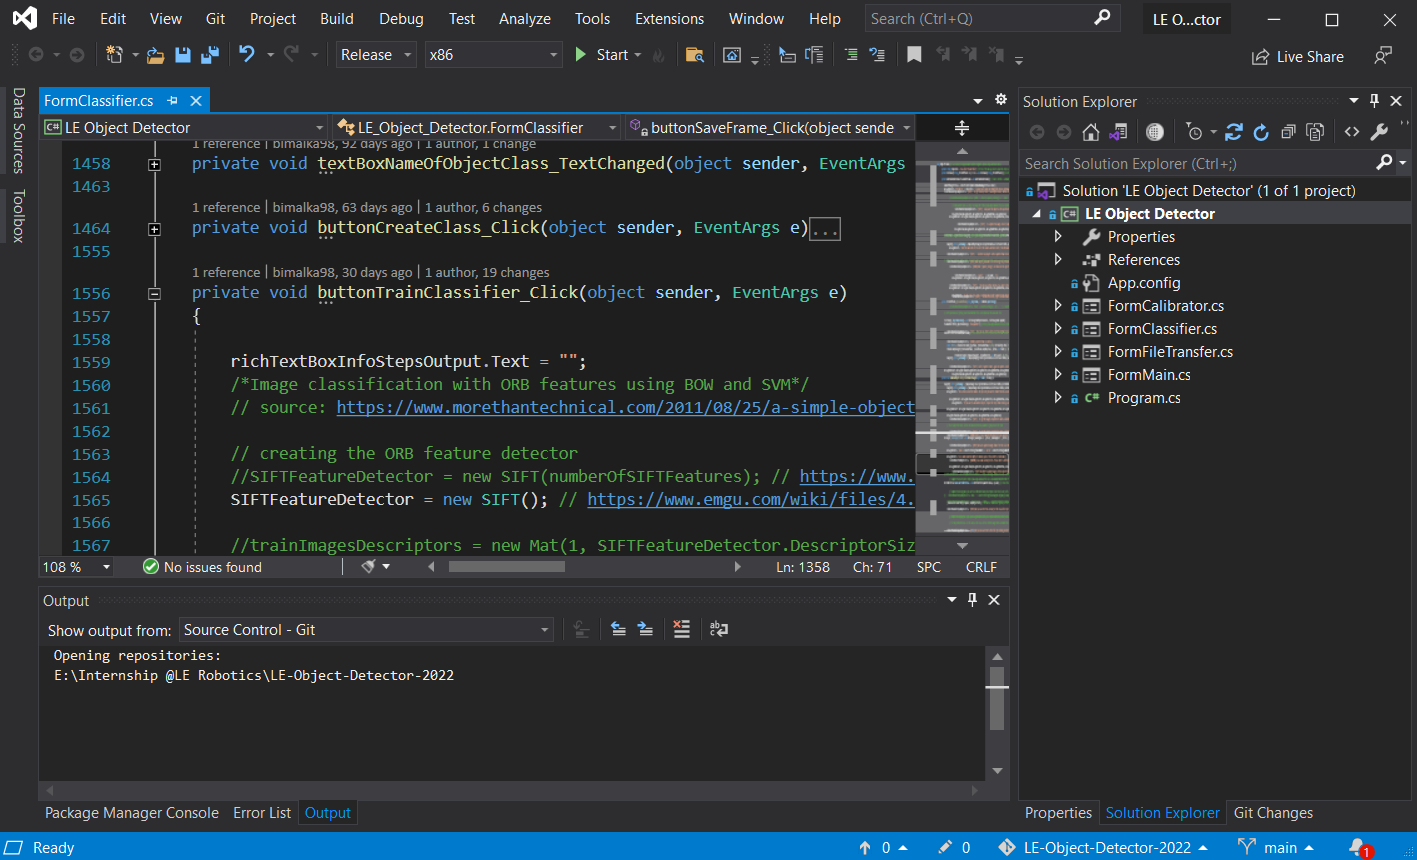
\includegraphics[width=0.8\linewidth]{figures/handson/vs}
	}
	\caption{``Visual Studio 2019'' \ac{ide}}
	\label{fig:vs}
\end{figure}

Visual Studio uses various Microsoft software development platforms to develop software. In my project I used what is known as \textit{Windows Forms} platform. It is a free and open-source \ac{gui} class library included as a part of Microsoft .NET Framework, providing a platform to write client applications for desktop, laptop, and tablet \ac{pc}s. An application developed using the Windows Forms platform is called as a \textit{Windows Forms Application}. These applications are event-driven applications which means they spends most of their time simply waiting for the user to do something, such as fill in a text box or click a button\cite{winforms}. The code for the applications developed by me were written in {\tt C\#} language.


\subsection{Visual Studio Code}

\textit{Visual Studio Code} is a lightweight \ac{oss}, which can be used to write/edit computer programs (source codes) efficiently. It is being developed by Microsoft with the help of thousands of other developers all over the world. It can run on your desktop and is available for Windows, macOS and Linux. It comes with built-in support for a few programming languages and has a rich ecosystem of extensions for other languages as well to customize it according to the needs of the developer. In short, this cool, powerful application is called as \textit{VS code} by the developers and Figure \ref{fig:vscode} shows an instance of the application.\\

\begin{figure}[H]
	\centering
	\fbox{
		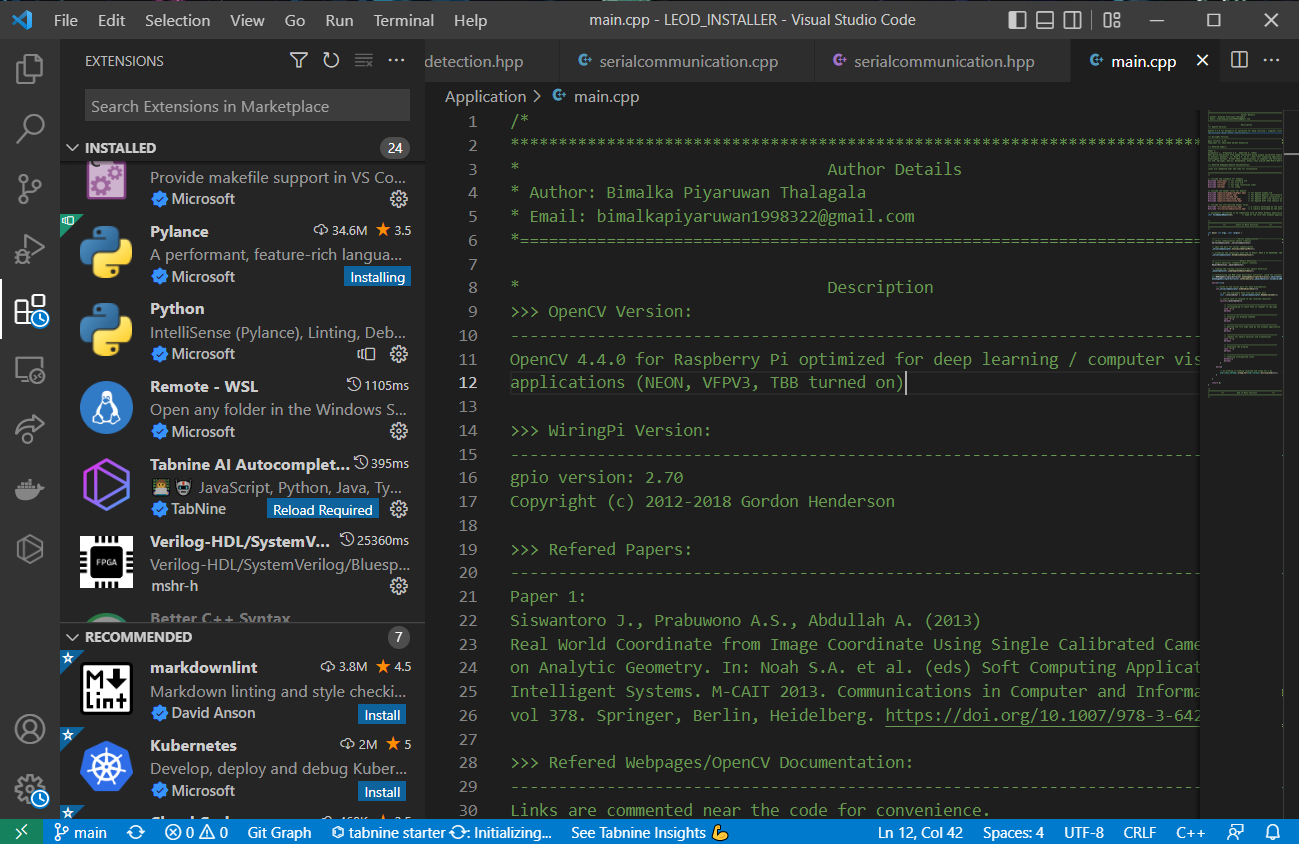
\includegraphics[width=0.82\linewidth]{figures/handson/vscode}
	}
	\caption{``Visual Studio Code'' source code editor}
	\label{fig:vscode}
\end{figure}

During my internship, I used VS code extensively for the development of the object detection framework described in Section \ref{Development of an Object Detection Framework}. I developed that algorithm using {\tt C++} language and the VS code extension for {\tt C/C++} was absolutely a game changer during the implementation. Some of the fascinating features of the VS code is given below\cite{vscode}.

\begin{itemize}
	\item \textit{IntelliSense}, which provides smart completions based on variable types, function definitions, and imported modules.
	
	\item Built-in debugger with breakpoints, call stacks, and interactive console features.
	
	\item Built-in version controlling services to keep track of every line of your code.
	
	\item Rich ecosystem of extensions for customization.
\end{itemize}



\subsection{Git}

If the project at hand is related to software development, \textit{Git} is a must-have tool that you should be aware of. The reason can be explained as follows. Imagine an application is being developed by you, and you have made it to a working and stable state. Now your client wants you to add a new feature to the existing application. However, you are uncertain whether the application would work after the addition of the requested feature. Therefore, you tend to make a copy of your stable source code and start working on that copy. Now all the changes are done related to the new feature and you have made it works somehow.\\

What if the client wants to make a few changes and test another new feature? You have to repeat the same cycle by copying the latest stable version of your application. Imagine, what would happen if your client requested you to update the application for 10 more features. You will end up having a bunch of copies of the previous versions and it becomes an absolute mess. As you have to remember what each copy does. This is where the amazing tool `git' comes into the picture. Its logo is shown in the Figure \ref{fig:git}.\\

\begin{figure}[h]
	\centering
	\fbox{
		
\includegraphics[width=0.4\linewidth]{figures/handson/git}
	}
	\caption{ Logo for Git (introduced in 2012)\cite{gitlogo}}
	\label{fig:git}
\end{figure}

Git records changes to a file or set of files over time so that you can recall specific versions later. Therefore, you only need to keep one project directory and there is no need of keeping several copies of the same application (folder). This can be seen as \textit{time travel through the history of a specific project/ file}. In this way, git allows you to revert selected files back to a previous state, revert the entire project back to a previous state, compare changes over time, see who last modified something that might be causing a problem, who introduced an issue and when, and more\cite{git}.


\subsection{CMake}

In my project, the software development of the object detection framework described in Section \ref{Development of an Object Detection Framework} was carried out on a Windows \ac{pc}. However, the final target platform to run that application was a \ac{rpi}, which has a Linux based \ac{os} named as \textit{Debian}. A software that is compiled for a  Windows \ac{os}, can not run on a Linux system. Therefore, a method to bridge this gap as well as to automate the software build process inside the \ac{rpi} was required. This is where, \textit{CMake} came into the picture. Its logo is shown in the Figure \ref{fig:cmake}.

\begin{figure}[h]
	\centering
	\fbox{
		
\includegraphics[width=0.3\linewidth]{figures/handson/cmake}
	}
	\caption{ Logo for CMake\cite{cmake}}
	\label{fig:cmake}
\end{figure}

CMake is a cross-platform, free and \ac{oss} for build automation, testing, packaging and installation of software by using a compiler-independent method. That is, CMake doesn't actually execute the build process; instead, it generates build files for other systems such as Linux or Windows. It supports directory hierarchies and applications that depend on multiple libraries\cite{cmakewiki}. In my projects CMake was used as a build automation tool for generating build files of the objects detection framework for \ac{rpi}'s \ac{os}.

\chapter{Soft Skills Development}

When it comes to the present corporate world, it is obvious that technical skills alone can not take anyone to greater heights in his career. A person must be a perfect combination of both technical and soft skills to grow in whatever field he is in. Learning a new technical skill is not a big deal with the advancements in technology as everything is available at the fingertip. However, mastering a soft skill is much harder and takes time as we have to deal with human beings to do so.\\

LE Robotics Pvt. Ltd. was absolutely an ideal place to improve existing soft skills as well as to learn a new set of soft skills. Given below is a few of them. Please note that they are not in any specific order.

\begin{itemize}
	\item Problem-solving  
	\item Adaptability
	\item Interpersonal skills 
	\item Project  management 
	\item Time management 
	\item Emotional intelligence
	\item Professional work ethic 
	\item Communication 
\end{itemize}

Few of the above listed soft skills and their relation to the industrial training that I have received from  LE Robotics \ac{rnd} facility is explained in the upcoming sections of this chapter.

\section{Problem solving} 

Solving problems is an art that needs to be mastered by every engineer regardless of his field. Problem-solving skills that I have gained in the university as an engineering undergraduate were a massive help for me to tackle the project work explained in Section \ref{Project Work}. During my internship, I could sharpen those skills to suit to industrial level with the guidance of my supervisor.\\

Solving a problem includes several stages such as identifying and formulating the problem, researching the literature to find out available solutions and analyzing them, designing components of the system and validating their functionalities and etc. Before joining LE robotics Pvt. Ltd. I did not have much knowledge about researching the literature to find out potential solutions. All I used to do at the university was googling to find solutions from here and there and combine them to make one solution fit the problem at hand.\\

However, I could realise, that method fails when it comes to the industry. This is where my supervisor guided me towards conducting substantial literature research based on `\textit{Research Publications}' which exposed me to the world of `\textbf{Research}'. Research publications are published by academic institutes, research laboratories and other renowned companies such as Google, Microsoft and etc. Therefore, the information on those publications is well documented and validated which makes them an ideal information source. In addition to that, their reliability is also very high as the authors are professionals in their respective fields.



\section{Adaptability} 

Companies and working environments are different from one another. To get the most out of where you are, you need to effectively adapt to the current environment and its people. Inability to do so can lead to various problems within the work environment and you can lose interest in working there.\\

One of the main challenges that I faced during the internship was not having an expert in the field I worked in, to get any useful advice. Because my supervisor was only capable of setting an end goal and providing a high-level solution which can have tons of solutions in the \ac{cv} literature. Moreover, he had no idea about the complexity of some of the assigned tasks. Due to the gap between what we learn at university and practical problems that arise when it comes to an industrial-level implementation, I was having a difficult time there in the first few weeks.\\

To receive some advice regarding this situation, I contacted one of the lecturers at our university. He provided me with some potential tricks to get out of the situation while keeping everyone happy. The best of those was ``work, for yourself'', not for anyone else, not for the company but for you. Because if you get mad and do nothing due to not receiving enough support, you are the one who is going to be adversely affected by it in the end. Therefore, I worked for myself and could complete my assigned task very well with the provided resources at the end.  



\section{Time management} 

There are several actions that can be taken to manage one's time effectively.  Proper planning and organization of the assigned tasks depending on their priority are crucial when it comes to proper time management. Because, if you can not plan and organize the assigned tasks you can be easily overwhelmed by them. During my internship, time management was not a problem for me due to the experience I have gained at university regarding the proper management of the available time. Moreover, the knowledge of modern tools that I had, to get various jobs done was also a plus point. Because, lack of knowledge of the correct tool to use for a particular purpose, can waste your time.

\section{Professional work ethic}
Respecting professional engineering work ethics is a must-have soft skill when it comes to the cooperative world. You may be a high performer but if you can not be trusted, it will adversely affect the long run in the industry. Therefore, to be successful in the industry you must have good technical performance as well as the best professional work ethic. Our supervisor taught us more professional ethics than technical skills. Because with the advancement of today's technology gaining a technical skill is more than easy. However, becoming a man with professional ethics takes time and experience. Some of the ethics I have learned during my internship are mentioned below.

\begin{itemize}
	\item Punctuality
	\item Trustworthiness and obeying the \ac{nda}s of the organization.
	\item Perform services only in the areas of competence.
	\item Having a mindset to complete the assigned tasks without limiting to working hours/ days.
	\item Respect the \ac{ip} of others.
	\item Paying special attention to the terms and conditions of the  Licenses of \ac{oss} when using them in applications.
\end{itemize}

\section{Communication}
Communication in an industrial environment can be defined as conveying or sharing ideas effectively and listening actively. Communication can happen in verbal, written or as a combination of both formats. During my internship, I could gain much experience in effective communication through project demonstrations, various presentations and technical documentation preparations.\\

Project demonstrations included demonstrations of the projects explained in Section \ref{Project Work}. There I had to measure the performance of the developed \ac{cv} subsystem according to the criteria that were specified by the supervisor and present them to him for receiving feedback for further development of the system. Technical documentation preparation included preparing three technical documents which are explained below.

\begin{enumerate}
	\item A `System Installation Guide' for the \ac{cv} subsystem depicted in the Figure \ref{fig:cvsubsys} and explained in the Section \ref{Project Work}. 
	
	\item A `Further Development Guide` for the object detection framework explained in Section \ref{Development of an Object Detection Framework}.
	
	\item A `User Manual' which explains how to use the software explained in Sections \ref{Development of an Application for Camera Calibration} and \ref{Development of an Application to Train an Object Classification Model}.
\end{enumerate}


Through these three technical documentation preparation, I could gain a strong knowledge about documenting project works. It improved my technical writing capabilities as well as professional document editing using \LaTeX ~ which is a software system for scientific/technical document preparation.



\chapter{SWOT Analysis of the organization and self}

\section{SWOT Analysis of the Organization}


\subsection{Strengths}

This section summarises the \textit{internal} factors of the organization I observed during my industrial training, which are \textit{helpful} to achieve its business objectives.

\begin{itemize}
	\item Great vision towards making the ``Made in Sri Lanka'' brand strong through products that match international standards. In addition to that, they use 100\% local talent for all of their product designing tasks which has opened the doors for local undergraduates/ professionals to experience a real engineering product development process.
	
	\item Decades of experience in the industrial electronic product development industry in Sri Lanka.
	\item Unparalleled \ac{rnd} of advanced technologies such as industrial servo motors and their drivers with 100\% product ownership.
\end{itemize}


\subsection{Weaknesses}

This section summarises the \textit{internal} factors of the organization I observed during my industrial training, which is \textit{harmful} to achieve its business objectives.

\begin{itemize}
	\item Heavily depends on the interns - when I was doing my internship there were only two full-time employees in the facility. However, there were three of our interns and there were no experts in the field I was working too. I believe that the project that I had undertaken could be easily solved by a professional with experience in a very short period of time.
	
	\item Well-being or the career growth of the 
	employees were not of their concern - Because during our internship period there were not any social activities or additional workshops/ learning opportunities to improve the wellness of its employees. Whereas this is a major concern of modern business organizations.
	
\end{itemize}


\subsection{Opportunities}

This section summarises the \textit{external} factors of the organization I observed during my industrial training, which are \textit{helpful} to achieve its business objectives.

\begin{itemize}
	\item Industrial automation is a fast-growing field with enormous applications. Moreover, most of the problems in this field are yet to be understood clearly and a lot of \ac{rnd} work is carried out all over the world.
	
	\item When it comes to the local market there are very few competitors who work with similar technologies that LE Robotics (Pvt.) Ltd. works on.
\end{itemize}


\subsection{Threats}

This section summarises the \textit{external} factors of the organization I observed during my industrial training, which are \textit{harmful} to achieve its business objectives.

\begin{itemize}
	\item Slow product development speed in a fast 
	moving industry - in order to survive in a fast-moving industry like industrial automation, companies should rapidly develop their products.
	
	\item When it comes to the global scale the technologies that LE Robotics (Pvt.) Ltd. works on are already fully understood and there are huge competitors who dominate the market such as ``\textit{KUKA}''\cite{enwiki:kuka} which ships their products worldwide.
\end{itemize}


\section{SWOT Analysis of Self}


\subsection{Strengths}

This section summarises the \textit{internal} factors of me I identified during my industrial training, which are \textit{helpful} to achieving my life goals.
\begin{itemize}
	\item Can work under minimum supervision - in my point of view, this is my greatest achievement of the six months of special industrial training. The training at  LE Robotics (Pvt.) Ltd. showed me my true potential as an engineering student.
	
	\item A team player with critical thinking abilities  
	
	\item Fast learner who learns as needed - with the strong fundamental knowledge of the various engineering principles we have learned in the university, it is not a big deal to grab various technologies fast. Moreover, with the advancement of technology, learning new technical skills is easier than ever.
\end{itemize} 


\subsection{Weaknesses}
This section summarises the \textit{internal} factors I identified during my industrial training, which are \textit{harmful} to achieving my life goals.
\begin{itemize}
	\item Underestimate myself when a new 
	challenge is introduced
	\item Can not tolerate any kind of injustice
\end{itemize} 


\subsection{Opportunities}
This section summarises the \textit{external} factors I identified during my industrial training, which are \textit{helpful} to achieving my life goals.
\begin{itemize}
	\item Industrial automation is a fast-growing field - every year enormous amount of job opportunities are made for fresh graduates with cutting-edge technological backgrounds.
	
	\item Professionals with both \ac{ai} and Embedded 
	Systems Engineering knowledge have a 
	higher demand - in order to develop intelligent embedded systems which need to work with minimum resources one has to have knowledge of both the engineering discipline mentioned before.
\end{itemize}


\subsection{Threats}
This section summarises the \textit{external} factors I identified during my industrial training, which are \textit{harmful} to achieving my life goals.
\begin{itemize}
	\item Below the average \ac{gpa} in the department - this was something that I could experience when we were applying for internships. Some companies have a tendency of shortlisting candidates solely depending on their \ac{gpa}.
	
\end{itemize} 







\chapter{Conclusion}


The special industrial training was a whole new challenge which demanded a different set of technical skills as well as soft skills. LE Robotics (Pvt.) Ltd. did a great job in injecting much of those during the period of six months. One of the best achievements of the training is the mindset that our supervisor built in us, towards working under minimum supervision. This gave me an opportunity to experience my full potential as an engineering student and revealed my true calibre. This definitely, will be massive support for me to thrive in the fast-moving industry rather than surviving there. Because what I could realize during the training period was that there will be no one to spoon-feed you in the industry and you have to learn things fast on your own.\\

As a trainee, I was assigned a project to develop a Computer Vision subsystem for a pick and place machine. Since there were no experts in the Computer Vision field in the facility, the entire prototype development process was done individually by myself. Therefore, I could gain a very strong knowledge about turning an idea into a viable prototype using the available resources in the facility. During that process, I went over the stages such as idea generation, research, planning and prototyping. I believe, the process could be accelerated by a large factor if there was an expert in the Computer Vision field.\\

In the last month of the training period, I had the opportunity to work with our supervisor and the other employees of the facility for integrating the developed Computer Vision subsystem with the existing six degrees of freedom articulated robot arm. This taught me the importance of being a team player and completing the assigned tasks well in advance, to be successful in the final stages of product development. Because the subsystems/ modules that are developed by you must be compatible with the subsystem/ modules developed by the other employees for the system to function as one single unit.\\

From the very beginning of our training period, we had been working and working with no breaks other than the mercantile holidays and some of the weekends. LE Robotics (Pvt.) Ltd. was busy getting the work done from their employees and the well-being or the career growth of the employees was not of their concerns. Because we could not experience any social activity or additional workshops/ learning opportunities to improve the wellness of its employees. This was a major weakness of the company that was observed during my internship. Therefore, I could experience a serious work-life imbalance during the training period which eventually make me lose interest in the company even though they have a great vision. 












% ====================================================================
\begin{appendices}
	\chapter{Camera Calibration} \label{Camera Calibration}
	
	The important input data needed for calibration of the camera is a set of 3D real world points and the corresponding 2D coordinates of these points in the image. 3D points are called object points and 2D image points are called image points.
	
	\begin{enumerate}[I.]
		\item \textbf{2D Image Points:} These points can be easily found from the images. These image points are the locations where two black squares touch each other in chess board. Functions in OpenCV is used to extract those points\cite{cam_calib:_nodate}.
		
		\item \textbf{Object Points:}  For simplicity, the chess board was kept stationary at XY plane, (so Z=0 always) and camera was moved accordingly. This consideration helps us to find only X,Y values. Now for X,Y values, we can simply pass the points as (0,0,0), (1,0,0), (2,0,0), ... which denotes the location of points. In this case, the results we get will be in the scale of size of chess board square\cite{cam_calib:_nodate}. But if we know the square size, (for our implementation square size of the chess board was 30 mm), we can pass the values as (0,0,0), (30,0,0), (60,0,0).
	\end{enumerate}
	
	The process of camera calibration is given below.
	
	\begin{enumerate}
		\item Keep the chess board stationary in the XY plane of the real world coordinate system as shown in the Figure \ref{fig:clib3dworld} and do not let it move due to any reason.
		
		\begin{figure}[h]
			\centering
			\fbox{
				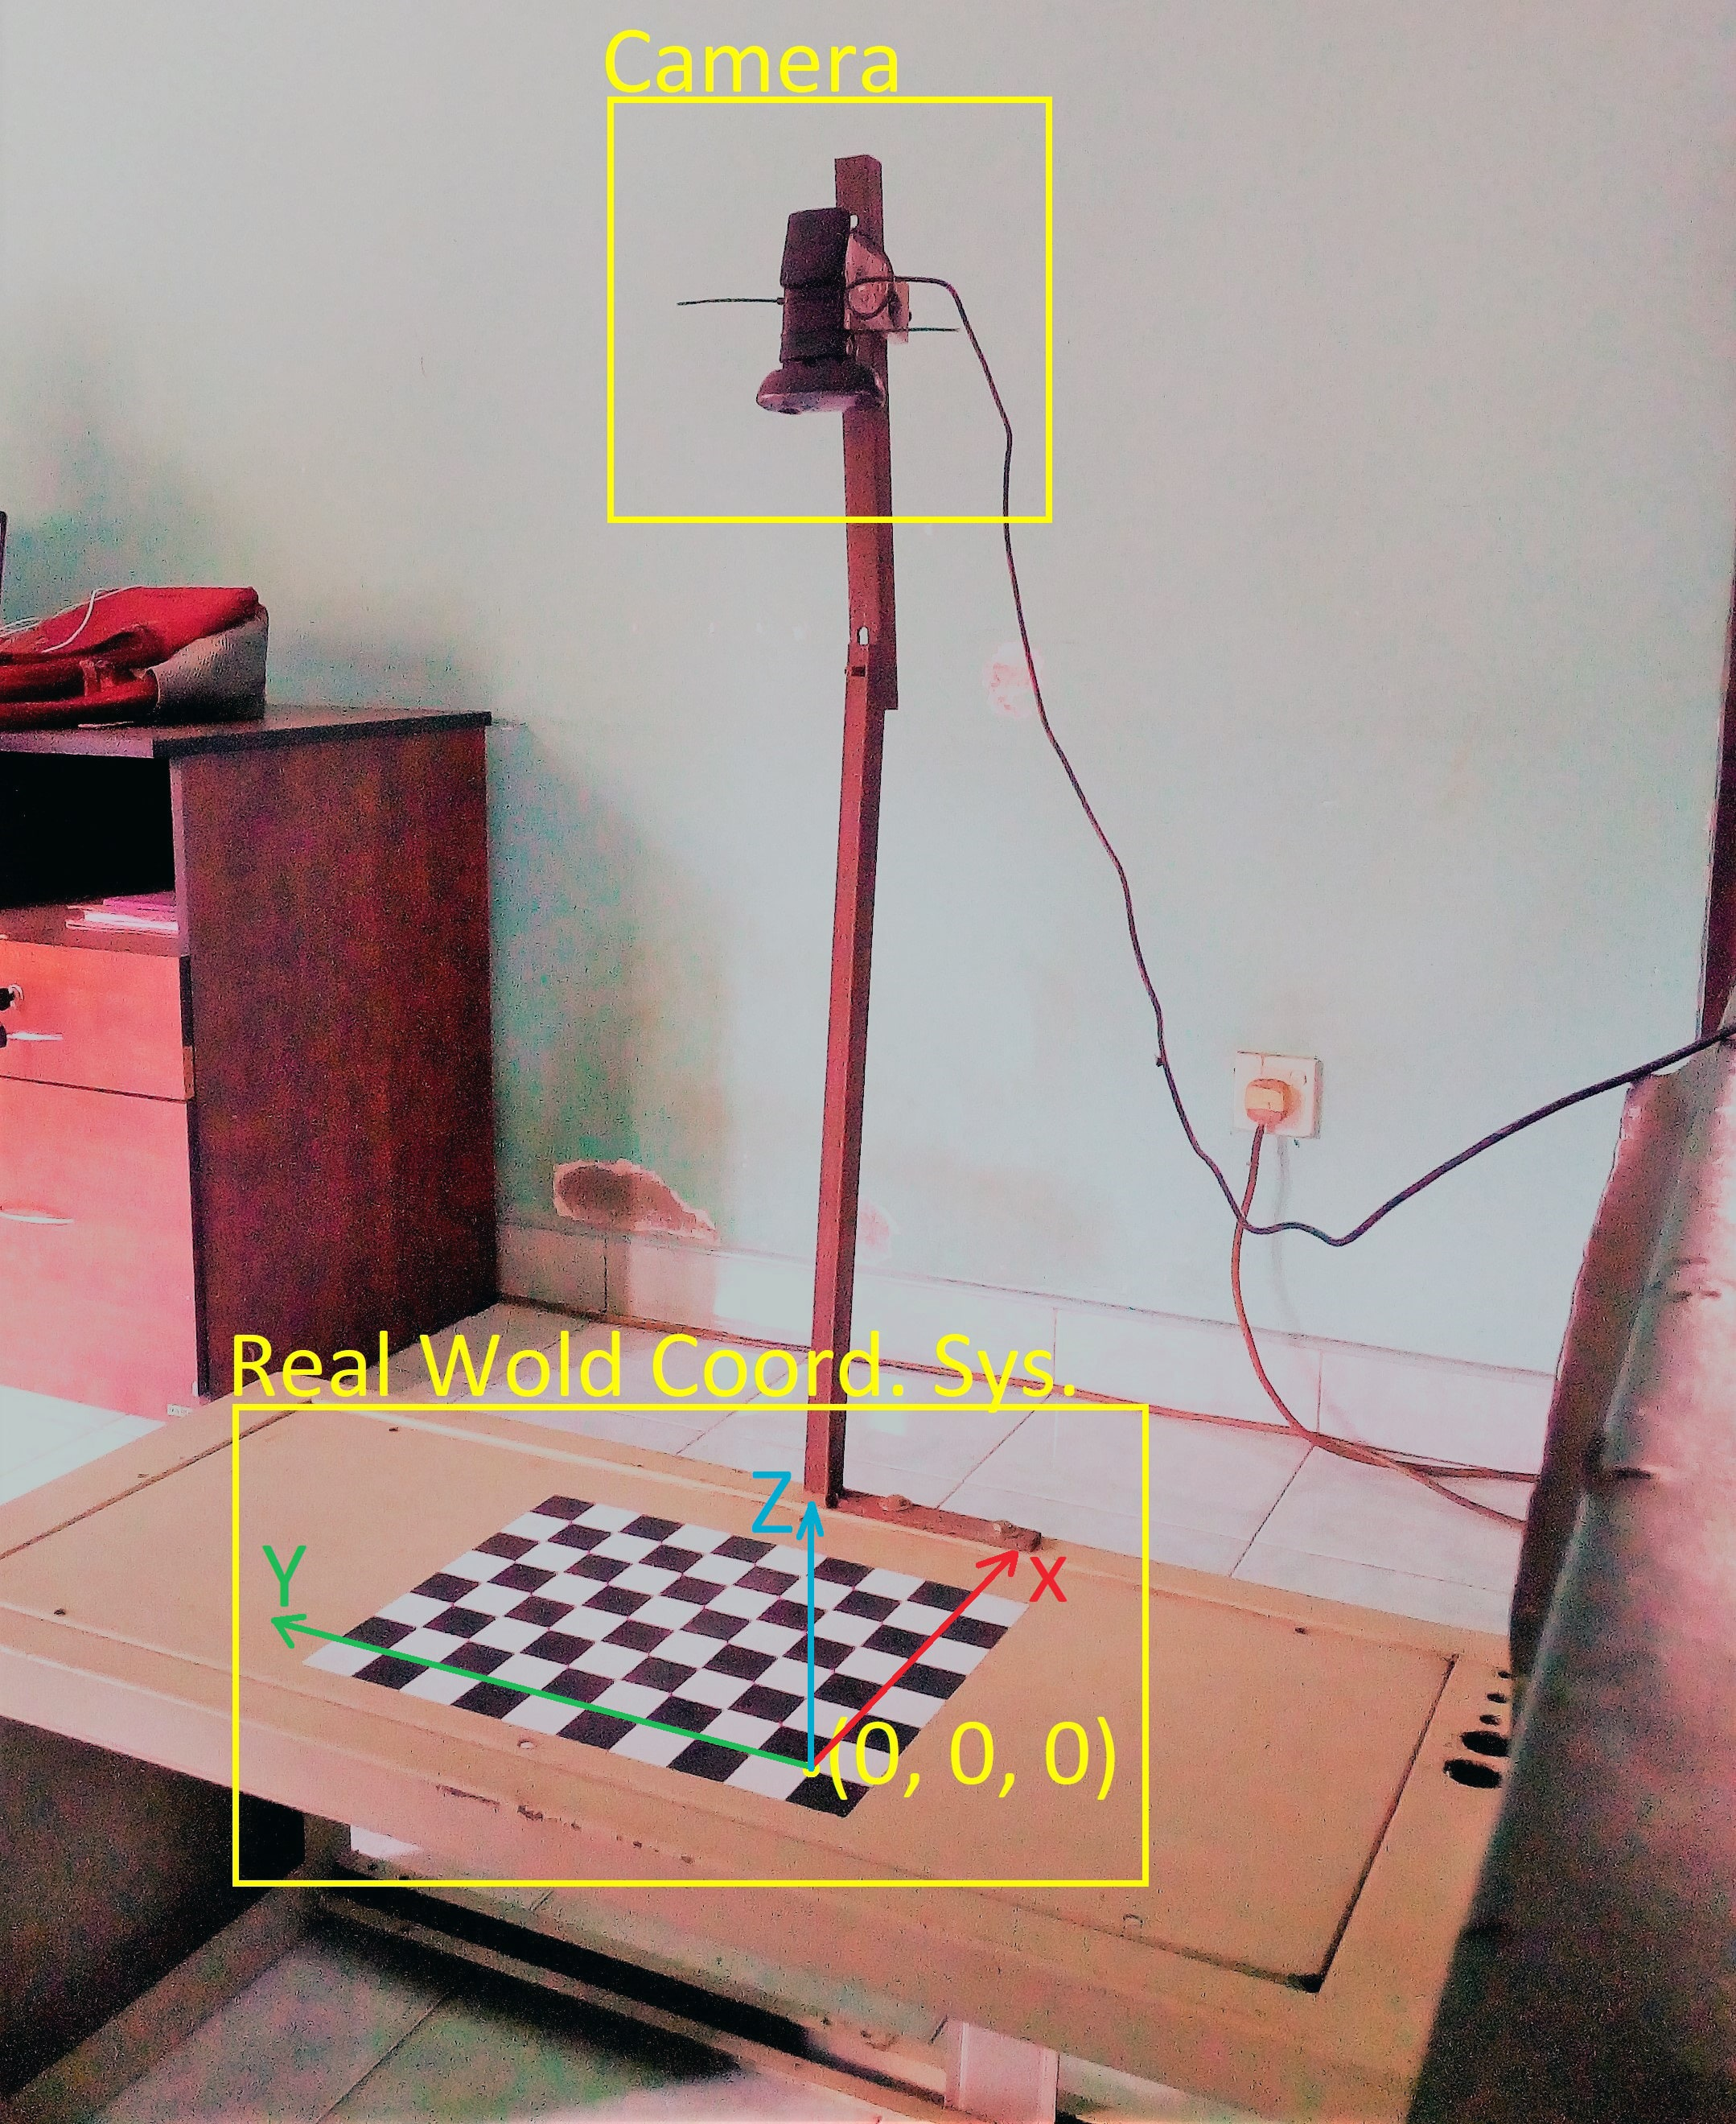
\includegraphics[width=0.35\linewidth]{figures/calib/realworld}
			}
			\caption{Real world coordinate system and the position of the camera with respect to it. }
			\label{fig:clib3dworld}
		\end{figure}
		
		\item Capture about 10-15 images (higher the better) as shown in the Figure \ref{fig:rawimages} using the camera that will be used for object detection, in several distances and orientations.\\
		
		The actual number of required images is around 6. However, in some scenarios OpenCV is unable to detect the chess board pattern properly in every image. Two of such reasons are given below.
		
		\begin{itemize}
			\item\textbf{Only a part of the chessboard is visible in the captured image}: For the program to work, whole chessboard must be visible in the captured image.
			
			\item \textbf{No proper lighting conditions}: if the environment that the  chessboard is placed, does not have proper lighting conditions application will not work as expected. Therefore make sure that the chessboard pattern receives enough light.
			
		\end{itemize}
		Hence, it's better to capture images more than the required amount so that we can filter out damaged/ useless images later. 
		
		\begin{figure}[h]
			\centering
			\fbox{
				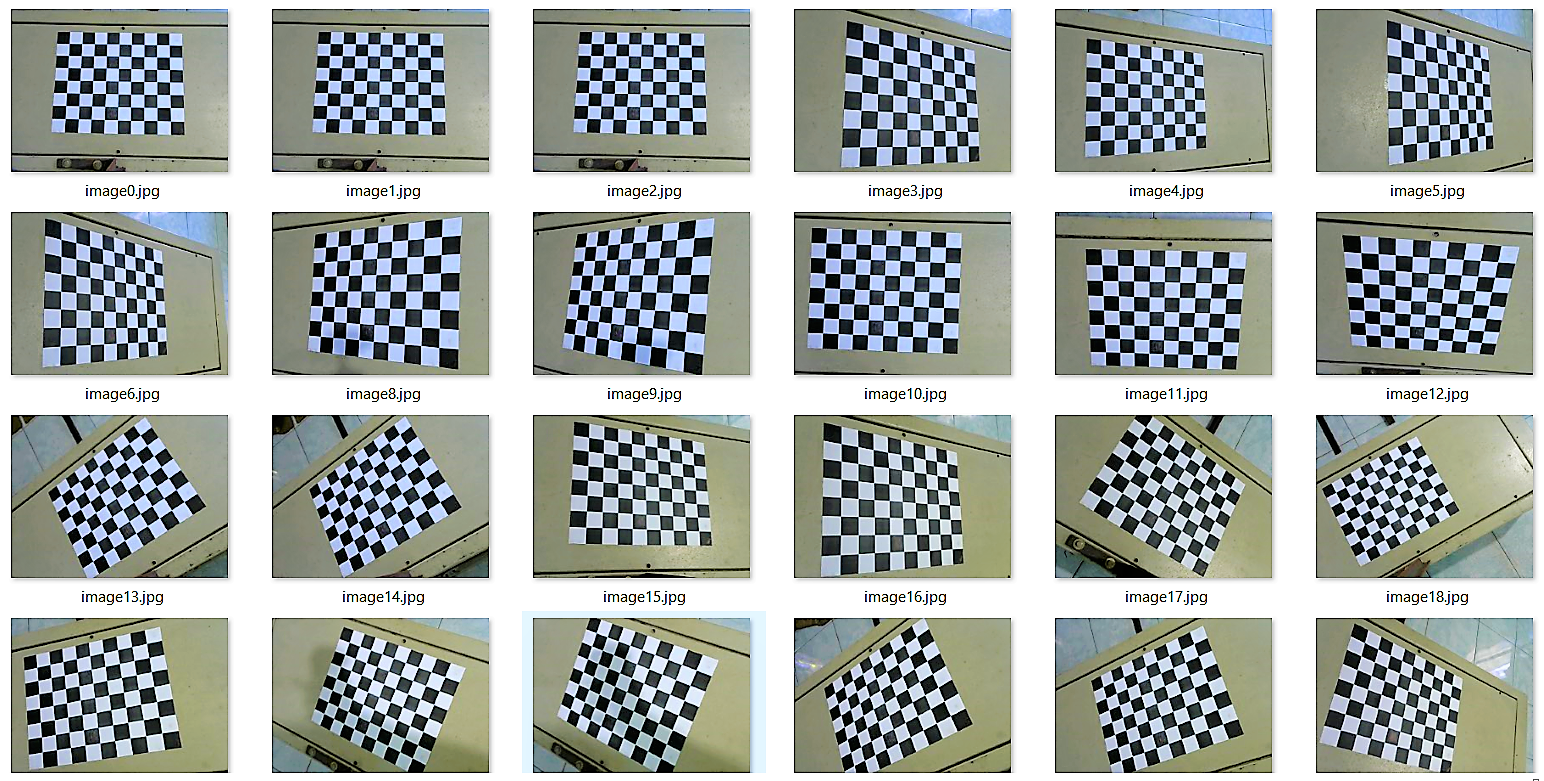
\includegraphics[width=0.8\linewidth]{figures/calib/rawImages}
			}
			\caption{Raw images captured by placing the camera in various distance and orientations}
			\label{fig:rawimages}
		\end{figure}
		
		\item Capture one additional special image, placing the camera in the place that it will be mounted when the actual object detection algorithm runs. Extrinsic parameters\cite{hartley_zisserman_2004} corresponding to this image will be directly used in our Back-projection algorithm.\\
		
		Extrinsic parameters contains a translation vector and a rotation matrix. These two together brings the calibration pattern from the object coordinate space (in which object points are specified) to the camera coordinate space. In more technical terms, the rotation matrix and translation vector performs a change of basis from object coordinate space to camera coordinate space. Due to its duality, it is equivalent to the position of the calibration pattern with respect to the camera coordinate space \cite{backproject:_nodate-1}.\\
		
		\begin{figure}[h]
			\centering
			\fbox{		\subfigure[Raw image]
				{ 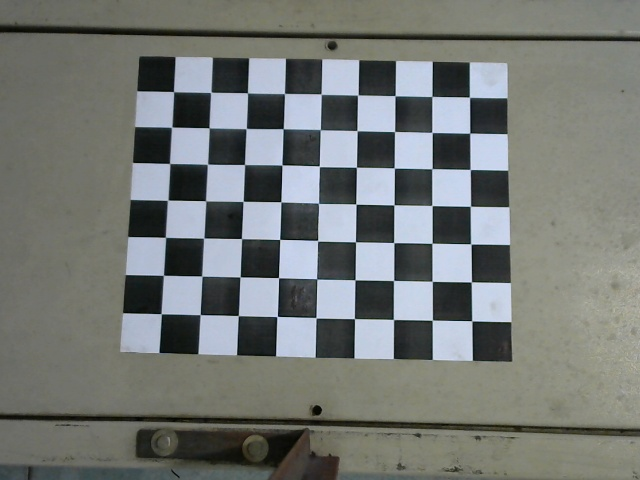
\includegraphics[scale=0.3]{figures/calib/image36}
					
				}\hfill
				\subfigure[Processed image to identify the pattern]
				{ 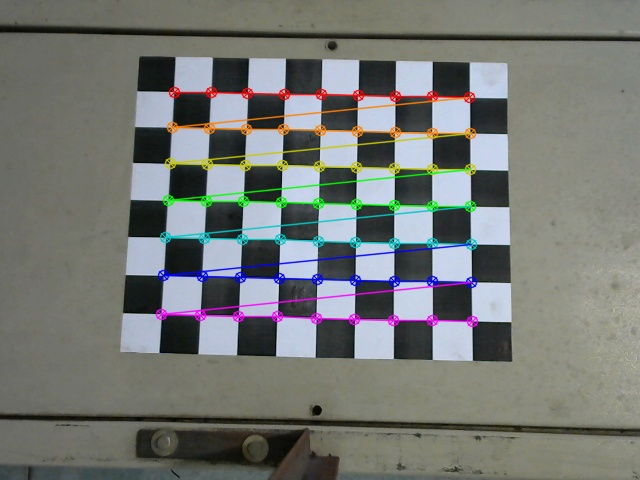
\includegraphics[scale=0.3]{figures/calib/image36proc}
					
			}}
			\caption{Captured special image to extract the extrinsic parameters that are useful for back-projection}
			\label{fig:backprojectimage}
		\end{figure}
		
		\item Use all of the captured images to calibrate the camera. The necessary documentation of the used functions are explained in \cite{backproject:_nodate-1}. After carrying out those functions you will be able to extract the extrinsic and intrinsic parameters related to the special image and the camera respectively.
	\end{enumerate}	
	
	
\end{appendices}

\footnotesize{
\twocolumn
\bibliographystyle{IEEEtrans}
\bibliography{refer}}

%---------------------------------------------------------------------------
\end{document}
-
